\chapter{Enhanced Sampling\label{chapter:ES}}
\begin{chapquote}{Bernard R. Brooks%, \textit{\url{https://en.wikiquote.org/wiki/Albert_Einstein}}
	}
	``Keep the smart guys around you.''
\end{chapquote}
From the definition, the free energy of a specific system is dominated by phase space regions with a low potential energy (metastable states). However, these regions might be separated by high energy barriers ($\gg k_BT$). Transitions among these potential energy wells are often hindered by these barriers. According to the Boltzmann's Law, the probability of a sample $\mathbf{R}$ being visited is proportional to the Boltzmann's factor $\exp{\left[-\beta E(\mathbf{R})\right]}$, where $\beta=1/k_BT$ is called the inverse temperature. $k_B$ is the Boltzmann constant and $T$ is the temperature. According to some experience, in a $100\, ns$ simulation, the system can overcome a barrier of $10\, k_BT$, which is $6\, kcal/mol$ at room temperature ($300\, K$). If the barrier is $1.5\, kcal/mol$ higher, it takes about $1\, \mu s$ (10 times longer) in average for the system to go over the barrier. If the barrier height reaches $9\, kcal/mol$, it takes $10\,\mu s$. And so on. 

With modern computers, the longest all-atom molecular dynamics simulation for biological systems is probably the one done by D.E. Shaw, which was on a time scale of 1 ms on a special-purpose computer ``Anton''. For most classical molecular dynamics simulations, the time scales are normally several $\mu s$ to tens of $\mu s$. For simulations using expensive Hamiltonians, such as in QM/MM simulations, the time scales that can be reached are usually three orders shorter. Clearly, molecular dynamics simulations are plagued by a timescale problem. In order to observe abundant transitions among these energy minima, which is required by free energy calculations, enhanced samplings are often indispensable. As shown in the Boltzmann's factor, the essential quantity that determines the rate of transitions is $\beta E$. In order to accelerate the phase space sampling, we can either increase the temperature or decrease the energy barrier. All the methods shown below can be classified into these two categories. Some recent review papers might help.\cite{ZuckermanARB2011,BernardiBBA2015,KamenikPCCP2022,ChenCOSB2022}
\clearpage 
% !TeX spellcheck = en_US
% !TeX encoding = UTF-8
\section{Replica Exchange Molecular Dynamics\label{Sec:ES:REMD}}
\subsection{Temperature-Replica Exchange Molecular Dynamics\label{Sec:ES:REMD:TREMD}}
Temperature replica exchange molecular dynamics (T-REMD) is one class of parallel tempering methods developed by Hansmann, Okamoto and Sugita\cite{HansmannJCC1993,HansmannCPL1997,SugitaCPL1999} based on many ideas in a category of methods called \textit{generalized-ensemble algorithm}. It is an extension of the well-known simulated annealing method. The basic idea of REMD is schematically summarized in Fig.~\ref{Fig:ES:REMD}. In REMD, the system is replicated into $\mathbf{M}$ \textit{non-interacting} copies (replicas). Each replica is coupled to a bath at temperature $T_m$, $(m=1,\dots,M)$. At a certain time, the system is at state X, which can be denoted as $X=\left(x_1^{[i(1)]},\dots,x_M^{[i(M)]}\right)=\left(x_{m(1)}^{[1]},\dots,x_{m(M)}^{[M]}\right)$. Here, we used $i$ and $m$ to label the replica and the temperature respectively. Because the replicas are non-interacting, the weight-factor for a state $X$ in this generalized ensemble is a direct product of the Boltzmann factors for each replica, i.e.
\begin{equation}
	W_{REM}(X)=\prod\limits_{m=1}^M\exp{\left(-\beta_m H\left(q^{[i(m)]},p^{[i(m)]}\right)\right)}=\prod\limits_{i=1}^M \exp{\left(-\beta_{m(i)}H\left(q^{[i]},p^{[i]}\right)\right)}\textsl{}
\end{equation}

\begin{figure}[htbp]
	\centering
	%	\resizebox{2cm}{!}{
	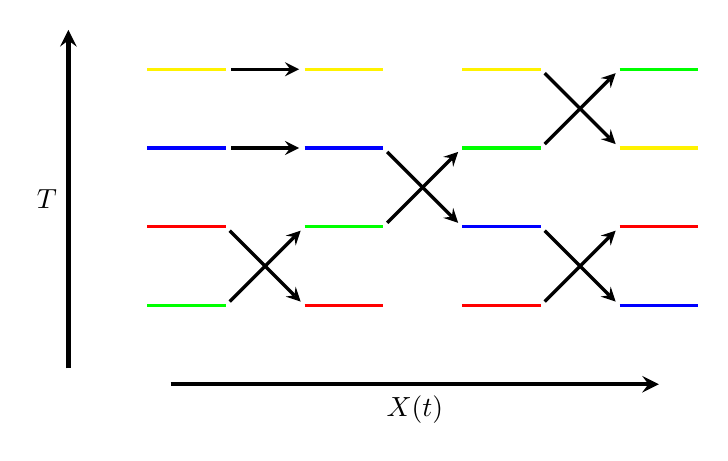
\begin{tikzpicture}
	    \draw[ultra thick,->,>=stealth] (1.3,0) -- (7.5,0) node[midway,below]{$X(t)$};
	    \draw[ultra thick,->,>=stealth] (0,0.2) -- (0,4.5) node[midway,left]{$T$};
	    
        \draw[very thick,green] (1,1) -- (2,1);
        \draw[very thick,red] (1,2) -- (2,2);
        \draw[very thick,blue] (1,3) -- (2,3);
        \draw[very thick,yellow] (1,4) -- (2,4);
        
        \draw[very thick,->,shorten >=2pt,shorten <=2pt,>=stealth] (2,1) -- (3,2);
        \draw[very thick,->,shorten >=2pt,shorten <=2pt,>=stealth] (2,2) -- (3,1);
        \draw[very thick,->,shorten >=2pt,shorten <=2pt,>=stealth] (2,3) -- (3,3);
        \draw[very thick,->,shorten >=2pt,shorten <=2pt,>=stealth] (2,4) -- (3,4);
        
        \draw[very thick,red] (3,1) -- (4,1);
        \draw[very thick,green] (3,2) -- (4,2);
        \draw[very thick,blue] (3,3) -- (4,3);
        \draw[very thick,yellow] (3,4) -- (4,4);
        
        \draw[very thick,->,shorten >=2pt,shorten <=2pt,>=stealth] (4,2) -- (5,3);
        \draw[very thick,->,shorten >=2pt,shorten <=2pt,>=stealth] (4,3) -- (5,2);
        
        \draw[very thick,red] (5,1) -- (6,1);
        \draw[very thick,blue] (5,2) -- (6,2);
        \draw[very thick,green] (5,3) -- (6,3);
        \draw[very thick,yellow] (5,4) -- (6,4);
        
        \draw[very thick,->,shorten >=2pt,shorten <=2pt,>=stealth] (6,1) -- (7,2);
        \draw[very thick,->,shorten >=2pt,shorten <=2pt,>=stealth] (6,2) -- (7,1);
        \draw[very thick,->,shorten >=2pt,shorten <=2pt,>=stealth] (6,3) -- (7,4);
        \draw[very thick,->,shorten >=2pt,shorten <=2pt,>=stealth] (6,4) -- (7,3);
        
        \draw[very thick,blue] (7,1) -- (8,1);
        \draw[very thick,red] (7,2) -- (8,2);
        \draw[very thick,yellow] (7,3) -- (8,3);
        \draw[very thick,green] (7,4) -- (8,4);        
	\end{tikzpicture}
	%	}
	\caption{A schematic representation of replica exchange molecular dynamics.}\label{Fig:ES:REMD}
\end{figure}

%\begin{figure}[htbp]
%    \centering
%	\includegraphics[width=0.6\textwidth]{figures/REMD.pdf}\\
%	\caption{A schematic representation of replica exchange molecular dynamics.}\label{Fig:ES:REMD}
%\end{figure}

Now, we exchange the temperatures of a pair of replicas
\begin{equation}
	\left\{ 
	\begin{array}{rcll} 
		x_m^{[i]}\equiv& \left(q^{[i]},p^{[i]}\right)_m \Rightarrow x_n^{[i]^\prime}&\equiv \left(q^{[i]},p^{[i]^\prime}\right)_n&\\ 
		&&&,\\
		x_n^{[j]}\equiv& \left(q^{[j]},p^{[j]}\right)_n \Rightarrow x_m^{[j]^\prime}&\equiv \left(q^{[j]},p^{[j]^\prime}\right)_m&\\  
	\end{array} 
	\right. 
\end{equation}
where
\begin{equation}
	\left\{ 
	\begin{array}{rl} 
		p^{[i]^\prime}\equiv \sqrt{\frac{T_n}{T_m}} p^{[i]}&\\ 
		&.\\
		p^{[j]^\prime}\equiv \sqrt{\frac{T_m}{T_n}} p^{[j]}&\\  
	\end{array} 
	\right. 
\end{equation}
The exchange rule is not trivial. In order for this exchange process to converge towards an equilibrium distribution, it is sufficient to impose the detailed balance condition on the transition probability $w(X\rightarrow X^\prime)$:
\begin{equation}
	W_{REM}(X)w(X\rightarrow X^\prime) = W_{REM}(X^\prime)w(X^\prime\rightarrow X).
\end{equation}
Then we have
\begin{align}
	&\frac{w\left(X\rightarrow X^\prime\right)}{w\left(X^\prime\rightarrow X\right)}\notag\\
	=&\frac{W_{REM}(X^\prime)}{W_{REM}(X)}\notag\\
	   =&\frac{\exp{\left(-\beta_m H\left(q^{[j]},p^{[j]^\prime}\right)\right)}\exp{\left(-\beta_n H\left(q^{[i]},p^{[i]^\prime}\right)\right)}}{\exp{\left(-\beta_m H\left(q^{[i]},p^{[i]^{ }}\right)\right)}\exp{\left(-\beta_n H\left(q^{[j]},p^{[j]^{ }}\right)\right)}}\notag\\
	   =&\frac{\exp{\left\{-\beta_m\left[K\left(p^{[j]^\prime}\right)+U\left(q^{[j]}\right)\right]-\beta_n\left[K\left(p^{[i]^\prime}\right)+U\left(q^{[i]}\right)\right]\notag\right\}}}
	   {\exp{\left\{-\beta_m\left[K\left(p^{[i]}\right)+U\left(q^{[i]}\right)\right]-\beta_n\left[K\left(p^{[j]}\right)+U\left(q^{[j]}\right)\right]\notag\right\}}}\notag\\
	   =&\frac{\exp{\left\{-\beta_m\left[\frac{T_m}{T_n}K\left(p^{[j]}\right)+U\left(q^{[j]}\right)\right]-\beta_n\left[\frac{T_n}{T_m}K\left(p^{[i]}\right)+U\left(q^{[i]}\right)\right]\notag\right\}}}
	   {\exp{\left\{-\beta_m\left[K\left(p^{[i]}\right)+U\left(q^{[i]}\right)\right]-\beta_n\left[K\left(p^{[j]}\right)+U\left(q^{[j]}\right)\right]\notag\right\}}}\notag\\
	   =&\dfrac{\exp{\left\{-\beta_n K\left(p^{[j]}\right)-\beta_m K\left(p^{[i]}\right)\right\}}}{\exp{\left\{-\beta_m K\left(p^{[i]}\right)-\beta_n K\left(p^{[j]}\right)\right\}}} \dfrac{\exp{\left\{-\beta_m U\left(q^{[j]}\right)-\beta_n U\left(q^{[i]}\right)\right\}}}{\exp{\left\{-\beta_m U\left(q^{[i]}\right)-\beta_n U\left(q^{[j]}\right)\right\}}}\notag\\
	   =&\exp{\left\{-\Delta\right\}}.
\end{align}
where $\Delta = \left[\beta_n-\beta_m\right]\left[U\left(q^{[i]}\right)-U\left(q^{[j]}\right)\right]$. It can be seen that the kinetic energy terms are fully canceled out.
This can be satisfied by the usual Metropolis criterion:
\begin{equation}
	w\left(X\rightarrow X^\prime\right)\equiv w\left(x_m^{[i]}\, \bigg\rvert\, x_n^{[j]}\right)= 
	\left\{ 
	\begin{array}{ll} 
		1, & \text{if } \Delta \leq 0\\ 
		\exp{(-\Delta)}, & \text{if } \Delta >0\\  
	\end{array} 
	\right. 
\end{equation}

The high-temperature replicas and the low-temperature replicas work in a collaborative way, in which the former explore phase space while the latter exploit phase space around local minima. After long time simulations, all the replicas have arrived at a global equilibrium. In order to calculate the free energy or the ensemble average of an operator $\hat A$ at $T_m$, we can extract all the snapshots that have a temperature $T_m$ from $M$ trajectories, if this temperature was among the $M$ chosen temperatures. However, the optimal way is to use Weighted Histogram Analysis Method in Section~\ref{Sec:FEM:WHAM} or the Multistate Bennett Acceptance Ratio method in Section~\ref{Sec:FEM:MBAR}.  

In the above derivation, it only considers exchanges between neighboring states. However, a global permutation is also possible, and sometimes it may improve sampling efficiency.\cite{ChoderaJCP2011}

\subsection{Hamiltonian-Replica Exchange Molecular Dynamics\label{Sec:ES:REMD:HREMD}}
Another type of REMD simulation is called Hamiltonian replica exchange molecular dynamics (H-REMD), in which each replicas has its own Hamiltonian, but is coupled to the same temperature.\cite{JangPRL2003} One example is the H-REMD simulation for a torsional angle. The $m$th replica has a torsional energy term of 
\begin{equation}
	H_m(\phi)=\lambda(m)\sum_n\left(V_n/2\right)\left(1+\cos{\left[n\phi-\delta\right]}\right),
\end{equation}
where $\lambda$ is a control parameter. $\lambda(0)=1$ corresponds to the unbiased state and at $\lambda(M)$ (usually $\lambda(M)=0$) the torsional motion of this dihedral angle has a smaller barrier.

Another example of HREMD is pH-REMD, in which each replica is coupled with different pH of the solution. In other words, the chemical potential of hydronium in each replica is different . Therefore, the protonation states (or probability of being protonated or deprotonated) of titratable residues in each replica may differ from those in other replicas. In the simulations, the protonation states of titratable residues have their protonation states alternated according to the Metropolis criterion
\begin{equation}
	P= 
	\left\{ 
	\begin{array}{ll} 
		1, & \text{if } \Delta G_{\ce{P_{A}}\rightarrow \ce{P_{A}H^{+}}}\leq 0\\ 
		\exp{(-\beta\Delta G_{\ce{P_{A}}\rightarrow \ce{P_{A}H^{+}}})}, & \text{if }\Delta G_{\ce{P_{A}}\rightarrow \ce{P_{A}H^{+}}} >0\\  
	\end{array} 
	\right. 
\end{equation}
using Monte Carlo. The derivation of $\Delta G_{\ce{P_{A}}\rightarrow \ce{P_{A}H^{+}}}$ is shown below. 

Free energy of molecule \ce{A} in solution with a concentration $\left[\ce{A}\right]$
can be written as 
\[
\Delta G_{\ce{A}}=\Delta G_{\ce{A}}^{0}+\beta^{-1}\ln\frac{\left[\ce{A}\right]}{C_{0}},
\]
in which $\Delta G_{\ce{A}}^{0}$ is the free energy of molecule A at the standard
state $C_{0}$, i.e. 1 mol/L. The free energy change for a reaction
\begin{center}
	\schemestart \chemfig{A} + \chemfig{B} \arrow{<=>}[,0.75] \chemfig{C} \schemestop
\end{center}
%\[
%A+B\rightleftharpoons C
%\]
can be written as
\[
\Delta G=\Delta G_{\ce{C}}-\Delta G_{\ce{A}}-\Delta G_{\ce{B}}=\Delta G_{0}+\beta^{-1}\ln\frac{\left[\ce{C}\right]C_{0}}{\left[\ce{A}\right]\left[\ce{B}\right]}.
\]

At equilibrium, the free energy change is zero, we have
\begin{equation}
	\Delta G_{0}=-\beta^{-1}\ln\frac{\left[\ce{C}\right]C_{0}}{\left[\ce{A}\right]\left[\ce{B}\right]},\label{eq:FEM:REMD:standardfreeenergy}
\end{equation}
in which $\left[\ce{A}\right]\left[\ce{B}\right]/\left[\ce{C}\right]C_{0}$ is called
the dissociation constant $K_{a}$. So,

\begin{equation}
\Delta G_{0}=\beta^{-1}\ln K_{a}.
\label{eq:FEM:REMD:standardfreeenergyvsKa}
\end{equation}

Titration of a residue in a real protein can be written as
\begin{center}
	\schemestart \chemfig{P_{A}} + \chemfig{H^{+}} \arrow{<=>}[,0.75] \chemfig{P_{A}H^{+}} \schemestop
\end{center}
%\[
%P_{A}+H^{+}\rightleftharpoons P_{A}H^{+},
%\]

with 
\[
K_{a}=\frac{\left[\ce{P_{A}}\right]\left[\ce{H^{+}}\right]}{\left[\ce{P_{A}H^{+}}\right]C_{0}}
\]

The fraction of the deprotonated species is calculated as

\begin{eqnarray}
	f_{\left[\ce{P_{A}}\right]} & = & \frac{\left[\ce{P_{A}}\right]}{\left[\ce{P_{A}}\right]+\left[\ce{P_{A}H^{+}}\right]}\nonumber \\
	& = & \frac{1}{1+\frac{\left[\ce{P_{A}H^{+}}\right]}{\left[\ce{P_{A}}\right]}}\nonumber \\
	& = & \frac{1}{1+\frac{\left[\ce{P_{A}}\right]\left[\ce{H^{+}}\right]}{C_{0}K_{a}\left[\ce{P_{A}}\right]}}\nonumber \\
	& = & \frac{1}{1+\frac{1}{C_{0}K_{a}}\left[\ce{H^{+}}\right]}\nonumber \\
	& = & \frac{1}{1+\frac{1}{K_{a}}10^{-\mathrm{pH}}}\label{eq:FEM:REMD:titrationcurve}
\end{eqnarray}
We can check the asymptotic behavior of this equation. At strong
acidic condition ($\mathrm{pH}=-\infty$), $f_{\left[\ce{P_{A}}\right]}=0$, indicating that
the residue is 100 percent protonated. While at an extremely basic
condition ($\mathrm{pH}=\infty$), $f_{\left[\ce{P_{A}}\right]}=1$. This residue is 100
percent deprotonated. From the Henderson–Hasselbalch (HH) equation, 
the $\mathrm{p}K_a$ can be determined by the $\mathrm{pH}$ of the state when 
$\left[\ce{P_{A}}\right]/\left[\ce{P_{A}H^{+}}\right]=1$

\begin{align}
	\mathrm{p}K_{a}  = & -\log{K_{a}}\notag\\
	 = & -\log{\frac{\left[\ce{P_{A}}\right]}{\left[\ce{P_{A}H^{+}}\right]}}-\log{\frac{\left[\ce{H^{+}}\right]}{C_{0}}}\notag\\
	 = & -\log{\frac{\left[\ce{P_{A}}\right]}{\left[\ce{P_{A}H^{+}}\right]}}+\mathrm{pH}.
	 \label{eq:FEM:REMD:pKa}
\end{align}
The $\mathrm{p}K_{a}$ of each residue in a dipeptide has been determined by
experiment. However, when this residue is located in a certain protein,
its $\mathrm{p}K_{a}$ is different from that in the dipeptide. The difference
is called the $\mathrm{p}K_{a}$ shift. Instead of measuring the $\mathrm{p}K_{a}$
for a residue in a protein, we are more interested in calculating/measuring
the titration curve, which is the fraction of the deprotonated state
as a function of pH. From Eq.~\ref{eq:FEM:REMD:titrationcurve}, $f_{\left[P_{A}\right]}$
can be easily calculated if we know $K_{a}$ or equivalently the standard
free energy change of protonation in Eq.~\ref{eq:FEM:REMD:standardfreeenergyvsKa}.
The standard free energy can be calculated from the partition functions
as

\begin{eqnarray*}
	\Delta G_{0} & = & -\beta^{-1}\ln\frac{Q_{\ce{P_{A}H^{+}}}}{Q_{\ce{P_{A}}}Q_{\ce{H^{+}}}}\\
	& = & -\beta^{-1}\ln\frac{\iint\exp(-\beta E_{\ce{P_{A}H^{+}}})\diff \mathbf{R}_{H}\diff \mathbf{R}_{o}}{Q_{\ce{H^{+}}}\int\exp(-\beta E_{\ce{P_{A}}})\diff \mathbf{R}_{o}},
\end{eqnarray*}
where $\mathbf{R}_{H}$ is the coordinates of the specific \ce{H} atom and the other degrees-of-freedom (DoF) are denoted as $\mathbf{R}_{o}$. Generally, the absolute value of $\Delta G_{0}$ is hardly computable. A relative protonation free energy $\Delta\Delta G$ is preferred and is more reliable. Theoretically, the reference state can be any state you like. But the protonation free energy of the dipeptide is often used. The reference protonation process can be written as
\begin{center}
	\schemestart \chemfig{A} + \chemfig{H^{+}} \arrow{<=>}[,0.75] \chemfig{AH^{+}} \schemestop
\end{center}
%\[
%A+H^{+}\rightleftharpoons AH^{+}.
%\]

The free energy change from the reference state is 

\begin{align}
	&\Delta\Delta G_{0}\nonumber\\
	= & \Delta G_{0}-\Delta G_{0}^{ref}\nonumber \\
	= & -\beta^{-1}\ln\frac{\iint\exp(-\beta E_{\ce{P_{A}H^{+}}})\diff \mathbf{R}_{H}\diff \mathbf{R}_{o}}{Q_{\ce{H^{+}}}\int\exp(-\beta E_{\ce{P_{A}}})\diff \mathbf{R}_{o}}\frac{Q_{\ce{H^{+}}}\int\exp(-\beta E_{\ce{A}})\diff \mathbf{R}_{o}}{\iint\exp(-\beta E_{\ce{AH^{+}}})\diff \mathbf{R}_{H}\diff \mathbf{R}_{o}}\nonumber \\
	= & -\beta^{-1}\ln\frac{\iint\exp(-\beta E_{\ce{P_{A}H^{+}}})\diff \mathbf{R}_{H}\diff \mathbf{R}_{o}\int\exp(-\beta E_{\ce{A}})\diff \mathbf{R}_{o}}{\int\exp(-\beta E_{\ce{P_{A}}})\diff \mathbf{R}_{o}\iint\exp(-\beta E_{\ce{AH^{+}}})\diff \mathbf{R}_{H}\diff \mathbf{R}_{o}}\nonumber \\
	= & -\beta^{-1}\ln\frac{\iint\exp{\left[-\beta \left(E_{\ce{P_{A}H^{+}}}^{bond}+E_{\ce{P_{A}H^{+}}}^{QM}+E_{\ce{P_{A}H^{+}}}^{ele}\right)\right]}\diff \mathbf{R}_{H}\exp\left(-\beta E_{\ce{P_{A}H^{+}}}^{other}\right)\diff \mathbf{R}_{o}}{\iint\exp\left[-\beta \left(\ce{E_{AH^{+}}}^{bond}+E_{\ce{AH^{+}}}^{QM}+E_{\ce{AH^{+}}}^{ele}\right)\right]\diff \mathbf{R}_{H}\exp\left(-\beta E_{\ce{AH^{+}}}^{other}\right)\diff \mathbf{R}_{o}}\nonumber \\
	 & \cdot\frac{\int\exp\left(-\beta E_{\ce{A}}\right)\diff \mathbf{R}_{o}}{\int\exp\left(-\beta E_{\ce{P_{A}}}\right)\diff \mathbf{R}_{o}},\label{eq:FEM:REMD:Quotientofpartitionfunctions}
\end{align}
where $E^{bond}$
and $E^{ele}$ are the bonded energy and electrostatic interaction
energy related to this \ce{H} atom, respectively. $E^{QM}$ is the energy
correction that \textit{may} be required if the molecular mechanical
Hamiltonian cannot well capture the energy of the system, such as
the missing of charge transfer effect. The sum of the remaining energy
term is denoted as $E^{other}$, which does not explicitly depend
on the position of this specific \ce{H} atom. Eq.~\ref{eq:FEM:REMD:Quotientofpartitionfunctions}
is not ready to be computed before some approximations are adopted. 

\textit{First}, we assume that the total energy can be well described by the MM Hamiltonians
for both the state interested in and the reference state. Therefore,
\[
E_{\ce{P_{A}H^{+}}}^{QM}=E_{\ce{AH^{+}}}^{QM}=Const,
\]
and they can be removed from the integral. 

\textit{Second}, the bonded terms involving hydrogen atoms are usually 
constrained in the simulations. Therefore, the hydrogen atom in question has 
only one position and $E^{bond}=0$. Now, the 
relative protonation free energy can be simplified as
\begin{align}
\Delta\Delta G_{0}=&-\beta^{-1}\ln\frac{\int\exp\left(-\beta E_{\ce{P_{A}H^{+}}}^{ele}\right)\exp\left(-\beta E_{\ce{P_{A}H^{+}}}^{other}\right)\diff \mathbf{R}_{o}}{\int\exp\left(-\beta E_{\ce{AH^{+}}}^{ele}\right)\exp\left(-\beta E_{\ce{AH^{+}}}^{other}\right)\diff \mathbf{R}_{o}}\notag\\
&\cdot\frac{\int\exp\left(-\beta E_{\ce{A}}\right)\diff \mathbf{R}_{o}}{\int\exp\left(-\beta E_{P_{\ce{A}}}\right)\diff \mathbf{R}_{o}}.
\end{align}

Note that $E_{\ce{A}}=E_{\ce{AH^{+}}}^{other}$ and $E_{\ce{P_{A}}}=E_{\ce{P_{A}H^{+}}}^{other}$, we have
\begin{align}
	\Delta\Delta G_{0} = & -\beta^{-1}\ln\frac{\int\exp\left(-\beta E_{\ce{P_{A}H^{+}}}^{ele}\right)\exp\left(-\beta E_{\ce{P_{A}}}\right)\diff \mathbf{R}_{o}}{\int\exp\left(-\beta E_{\ce{P_{A}}}\right)\diff \mathbf{R}_{o}}\\
	& \cdot \frac{\int\exp\left(-\beta E_{\ce{A}}\right)\diff \mathbf{R}_{o}}{\int\exp\left(-\beta E_{\ce{AH^{+}}}^{ele}\right)\exp\left(-\beta E_{\ce{A}}\right)\diff \mathbf{R}_{o}}\\
	= & -\beta^{-1}\ln\left\langle \exp\left(-\beta E_{\ce{P_{A}H^{+}}}^{ele}\right)\right\rangle _{\ce{P_{A}}}\notag\\
	  &+\beta^{-1} \ln\left\langle \exp\left(-\beta E_{\ce{AH^{+}}}^{ele}\right)\right\rangle _{\ce{A}}\notag\\
	= & \Delta G_{\ce{P_{A}H^{+}}}^{ele}-\Delta G_{\ce{AH^{+}}}^{ele}  
\end{align}

Therefore,
\[
-\beta^{-1}\ln10\cdot \mathrm{p}K_{a}=\Delta G_{\ce{P_{A}H^{+}}}^{ele}-\Delta G_{\ce{AH^{+}}}^{ele}-\beta^{-1}\ln10\cdot \mathrm{p}K_{a}^{ref}.
\]

Using Eq.~\ref{eq:FEM:REMD:pKa}, at a certain pH the free energy difference between the deprotonated
and the protonated state can be written as

\[
\Delta G_{\ce{P_{A}}\rightarrow \ce{P_{A}H^{+}}}=\Delta G_{\ce{P_{A}H^{+}}}^{ele}+\beta^{-1}(\mathrm{pH}-\mathrm{p}K_{a}^{ref})\ln10-\Delta G_{\ce{AH^{+}}}^{ele}.
\]

In the above equation, $\Delta G_{\ce{AH^{+}}}^{ele}$ can be obtained from a free energy calculation of the model system by alchemically annihilation of the proton. However, $\Delta G_{\ce{P_{A}H^{+}}}^{ele}$ is unknown. Approximately, it can be replaced with $\Delta H_{\ce{P_{A}H^{+}}}^{ele}$ averaged over a few snapshots.\cite{MengJCTC2010} In order to accelerate the convergence,
this pH-REMD is often coupled with other enhanced simulation methods, such as T-REMD\cite{MengJCTC2010} and EDS-REMD\cite{LeeJCTC2014} (see section~\ref{Sec:ES:EDS}).
\clearpage
\input {chapters/SimulatedTempering.tex}
\clearpage
% !TeX spellcheck = en_US
% !TeX encoding = UTF-8
\section{Umbrella Sampling\label{Sec:ES:US}}
Umbrella Sampling method was proposed by Torrie and Valleau in 1977,\cite{TorrieJComputP1977} and is still widely used nowadays.
Suppose we are studying a transition process between two states such as conversion between two dominant conformations or a chemical reaction, and these two states are separated by a high barrier relative to $k_BT$. Therefore, the transition is a rare event. A schematic representation of the free energy landscape is shown in Fig.~\ref{Fig:ES:dual_harmonic}.
\begin{figure}[htbp]
	\centering
%	\resizebox{2cm}{!}{
		\begin{tikzpicture}
		\def\lims{xmin=-5,xmax=5,ymin=-38,ymax=14}
		\begin{axis}[\lims,hide x axis, hide y axis,width=0.65\textwidth,height=0.4\textwidth]
           \addplot[mark=none,smooth,domain=-5:5] {0.4*((x+2)*(x-2))*((x+2)*(x-2))-2*(x+0.5)*(x+0.5)-4};
           \draw[solid,->,>=Latex] (axis cs:-5,-29)--(axis cs:5,-29) node[below]{$\xi$};
		\end{axis}
		\end{tikzpicture}
%	}
	\caption{A typical free energy surface. Two free energy wells are separated by a barrier higher than $k_BT$.}\label{Fig:ES:dual_harmonic}
\end{figure}

%\begin{figure}[htbp]
%	\centering
%	\includegraphics[width=0.6\textwidth]{figures/dual_harmonic.pdf}\\
%	\caption{A typical free energy surface. Two free energy barriers are separated by a barrier higher than $kT$.}\label{Fig:ES:dual_harmonic}
%\end{figure}

Sometimes, we are interested in not only these two dominant states but also the whole pathway. Usually, we define a reaction coordinate $\xi$, including one or more collective variables (CVs), which can distinguish the two minima and characterize the free-energy pathway. Then we want to know the free-energy change along the reaction coordinate, $\xi$. It should be noted that choosing a suitable set of CVs is nontrivial for most cases.\cite{LeitoldJCP2020} A CV can be either a real coordinate such as the difference of bond lengths in, for example, an $S_N2$ reaction, or a thermodynamics coupling parameter ($\lambda$) that defines an unphysical path. If we run a simulation with the reaction coordinate set to a local maximum, i.e. the system being the transition state, the system will quickly roll back to the ``reactant'' or the ``product'' state in order to reduce the free energy. The consequence is that phase space outside the ``reactant'' and ``product'' regions cannot be sampled sufficiently to yield accurate free energy profile in a brute force simulation. In order to enhance the exploration in these regions, we can added a bias potential $\Delta V(\xi)$ into the system, guaranteeing
\begin{equation}
	\forall \xi_{1} \; \mathrm{and} \; \xi_{2}, \left [ U(\xi_{1}) + \Delta V(\xi_{1}) \right ]  - \left [ U(\xi_{2}) + \Delta V(\xi_{2}) \right ] < k_BT
\end{equation}
then the free-energy surface can be explored within the timescale amenable to MD simulations. $\Delta V(\xi)$ is called the ``umbrella potential''.

However, as the free-energy surface is usually not known \textit{a priori}, it is difficult to determine $\Delta V(\xi)$. To circumvent this issue, we can stratify the free-energy pathway into multiple \textit{windows}, namely break up the reaction-coordinate space into ``parts'', by a series of (usually harmonic) restraints, $\Delta U_i(\xi)$. In other words, the $i$th simulation, or the simulation of the $i$th window, is performed on the potential energy surface 
\begin{equation}
	U_i(\mathbf{R})=U_0(\mathbf{R})+\Delta U_i(\xi).
\end{equation}
The strengths of the biases should be strong enough to maintain the system in the vicinity of where you are interested in, and also should be weak enough that the system can have significant overlap between two adjacent windows. At the same time, the windows should be small enough to guarantee in each window,
\begin{equation}
	\forall \xi_{1} \; \mathrm{and} \; \xi_{2}, \left [ U(\xi_{1}) + \Delta U_i(\xi_{1}) \right ]  - \left [ U(\xi_{2}) + \Delta U_i(\xi_{2}) \right ] < k_BT
\end{equation}
After all the simulations, the (biased) distribution of the samples in the whole region should be as flat as possible. Ensemble average under $U_0$ can be calculated from the ensembles generated under the biased Hamiltonians $U$ via
\begin{align}
	\left<X(\mathbf{R})\right>_0=&\frac{\int X(\mathbf{R})\exp{\left[-\beta U_0(\mathbf{R})\right]}\diff\mathbf{R}}{\int \exp{\left[-\beta U_0(\mathbf{R})\right]}\diff\mathbf{R}}\notag\\
	                            =&\frac{\int X(\mathbf{R})\exp{\left[\beta \Delta U_i(\mathbf{R})\right]}\exp{\left[-\beta U_i(\mathbf{R})\right]}\diff\mathbf{R}}{\int \exp{\left[\beta \Delta U_i(\mathbf{R})\right]}\exp{\left[-\beta U_i(\mathbf{R})\right]}\diff\mathbf{R}}\notag\\
	                =&\frac{\left<X\exp{\left(\beta\Delta U_i\right)}\right>_i}{\left<\exp{\left(\beta\Delta U_i\right)}\right>_i}.
	\label{Eq:ES:US:reweighting}
\end{align}
Better postprocessing methods are the Weighted Histogram Analysis Method, Umbrella Integration and the Multistate Bennett Acceptance Ratio method (to be discussed in Section~\ref{Sec:FEM:WHAM}, ~\ref{Sec:FEM:UI} and~\ref{Sec:FEM:MBAR}).
\clearpage
% !TeX spellcheck = en_US
% !TeX encoding = UTF-8
\section{Accelerated Molecular Dynamics\label{Sec:ES:aMD}}
Accelerated molecular dynamics, or aMD for short, was proposed by Hamelberg et al in 2004.\cite{HamelbergJCP2004}

In this method, the simulation is performed on the modified potential $V^\ast(\mathbf{r})$
\begin{equation}
	V^\ast(\mathbf{r})= 
	\left\{ 
	\begin{array}{rl} 
		V(\mathbf{r}), &\quad V(\mathbf{r})\geq E\\ 
		V(\mathbf{r})+\Delta V(\mathbf{r}), &\quad V(\mathbf{r})< E\\  
	\end{array} 
	\right.
\end{equation}
in which $E$ is a certain chosen energy, $\Delta V(\mathbf{r})$ is a continuous non-negative boost potential function, and $V(\mathbf{r})$ is the true potential. The bias potential increases the escape rate of the system from potential basins, and the subsequent state to state evolution of the system on the modified potential occurs at an accelerated rate with a nonlinear time scale of $\Delta t^\ast_i$, where
\begin{equation}
	\Delta t^\ast_i=\Delta t_i e^{\beta \Delta V(\mathbf{r}(t_i))}.
\end{equation}
The ensemble average value of any observable $A(\mathbf{r})$ taken on the modified potential can be written as
\begin{align}
	\left<A^\ast\right>=&\frac{\int \diff \mathbf{r}\,A(\mathbf{r})e^{-\beta V^{\ast}(\mathbf{r})}}{\int \diff \mathbf{r}\, e^{-\beta V^{\ast}(\mathbf{r})}}\notag\\
	        =&\frac{\int \diff \mathbf{r}\,A(\mathbf{r})e^{-\beta V(\mathbf{r})-\beta \Delta V(\mathbf{r})}}{\int \diff \mathbf{r}\, e^{-\beta V(\mathbf{r})-\beta \Delta V(\mathbf{r})}}.
\end{align}
The correct ensemble average can be written as
\begin{align}
	\left<A\right>=&\frac{\int \diff \mathbf{r}\,A(\mathbf{r})e^{-\beta V(\mathbf{r})}}{\int \diff \mathbf{r}\, e^{-\beta V(\mathbf{r})}}\notag\\
	=&\frac{\int \diff \mathbf{r}\,A(\mathbf{r})e^{-\beta V^\ast(\mathbf{r})+\beta \Delta V(\mathbf{r})}}{\int \diff \mathbf{r}\, e^{-\beta V^\ast(\mathbf{r})+\beta \Delta V(\mathbf{r})}}\notag\\
	=&\frac{\left<A(\mathbf{r})e^{\beta \Delta V(\mathbf{r})}\right>_{V^\ast}}{\left<e^{\beta \Delta V(\mathbf{r}) }\right>_{V^\ast}}.
\end{align}
Some technique can improve the numerical stability of this reweighting process.\cite{MiaoJCTC2014} The definition of $\Delta V(\mathbf{r})$ is non-unique, and Hamelberg et al proposed a modification of the potential energy surface more akin to snow drifts, which smooths the landscape by filling minima, but maintains the underlying shape of the unmodified potential energy surface and merges smoothly with the original potential at the threshold ``boost energy'' value $E$. It is defined as
\begin{equation}
	\Delta V(\mathbf{r})=\frac{(E-V(\mathbf{r}))^2}{\alpha+(E-V(\mathbf{r}))},
\end{equation}
where $\alpha$ is a tuning parameter that determines how deep the modified potential energy basin is (when $E-V(\mathbf{r})=\alpha, \Delta V(\mathbf{r})=\alpha/2$). With this biasing potential, the derivative of $V^{\ast}(\mathbf{r})$ has no discontinuity, and the modified potential reproduces the shape of the minima even at high value of $E$. Furthermore, $E$ should be carefully chosen, which may require a short trial simulation.

The most recent variant of aMD, the Gaussian accelerated molecular dynamics (GaMD), was developed by Miao et al\cite{MiaoJCTC2015}, in which the biasing potential is defined as
\begin{equation}
	\Delta V(\mathbf{r})= 
	\left\{ 
	\begin{array}{rl} 
		\frac{1}{2}k(E-V(\mathbf{r}))^2, &\quad V(\mathbf{r})< E\\ 
		0, &\quad V(\mathbf{r})\geq E\\  
	\end{array} 
	\right.
\end{equation}

In order to smoothen the potential energy surface for enhanced sampling, the boost potential needs to satisfy the following criteria. First, for any two arbitrary potential values $V(\mathbf{r}_1)$ and $V(\mathbf{r}_2)$ found on the original energy surface, $\Delta V$ should be a monotonic function that does no change the relative order of the biased potential values, i.e. 
\begin{equation}
	\sign{(V(\mathbf{r}_1)-V(\mathbf{r}_2))}=\sign{(V^\ast(\mathbf{r}_1)-V^\ast(\mathbf{r}_2))}.
\end{equation}
Without losing generality, let $V(\mathbf{r}_1)<V(\mathbf{r}_2)$, we have
\begin{equation}
	V^\ast(\mathbf{r}_1)<V^\ast(\mathbf{r}_2),
\end{equation}
which leads to
\begin{align}
    V(\mathbf{r}_1)+\frac{1}{2}k\left[E-V(\mathbf{r}_1)\right]^2-V(\mathbf{r}_2)-\frac{1}{2}k\left[E-V(\mathbf{r}_2)\right]^2<&0\notag\\
    \left[V(\mathbf{r}_1)-V(\mathbf{r}_2)\right]+\frac{1}{2}k\left[(2E-V(\mathbf{r}_1)-V(\mathbf{r}_2))(V(\mathbf{r}_2)-V(\mathbf{r}_1))\right]<&0\notag\\
    \left[V(\mathbf{r}_1)-V(\mathbf{r}_2)\right]\left[1-\frac{1}{2}k(2E-V(\mathbf{r}_1)-V(\mathbf{r}_2))\right]<&0.
\end{align}
Since $V(\mathbf{r}_1)<V(\mathbf{r}_2)$, we have
\begin{equation}
	1-\frac{1}{2}k(2E-V(\mathbf{r}_1)-V(\mathbf{r}_2))>0,
\end{equation}
or equivalently
\begin{equation}
	\text{Criterion 1: } E<\frac{1}{k}+\frac{1}{2}\left[V(\mathbf{r}_1)+V(\mathbf{r}_2)\right].
\end{equation}

Second, if $V(\mathbf{r}_1)<V(\mathbf{r}_2)$, the potential difference observed on the smoothened energy surface should be smaller than that of the original; i.e., $V^\ast(\mathbf{r}_2)-V^\ast(\mathbf{r}_1)<V(\mathbf{r}_2)-V(\mathbf{r}_1)$, which leads to
\begin{equation}
	\text{Criterion 2: } E>\frac{1}{2}\left[V(\mathbf{r}_1)+V(\mathbf{r}_2)\right].
\end{equation}
Therefore, the threshold energy must satisfy
\begin{equation}
	V_{\mathrm{max}}\leq E \leq V_{\mathrm{min}}+\frac{1}{k},
\end{equation}
where $V_{\mathrm{max}}$ and $V_{\mathrm{min}}$ are the maximum and minimum of potential energies, and $k$ has to satisfy
\begin{equation}
	k\leq \frac{1}{V_{\mathrm{max}}-V_{\mathrm{min}}}.
\end{equation}
It can be rewritten as
\begin{equation}
	k=k_0\frac{1}{V_{\mathrm{max}}-V_{\mathrm{min}}},
\end{equation}
where $k_0\in (0,1)$. $k_0$ determines the magnitude of the applied boost potential. With greater $k_0$, higher boost potential is added to the potential energy surface. The boost potential is
\begin{equation}
	\Delta V(\mathbf{r})=\frac{1}{2} k_{0} \frac{1}{V_{\max }-V_{\min }}(E-V(\mathbf{r}))^{2}, \quad V(\mathbf{r})<E.
\end{equation}

Third, the standard deviation of $\Delta V$ needs to be small enough (i.e., narrow distribution) to ensure accurate reweighting using cumulant expansion to the second order:\cite{MiaoJCTC2014}
\begin{equation}
	\sigma_{\Delta V}=\sqrt{\left(\left.\frac{\partial \Delta V}{\partial V}\right|_{V=V_{\mathrm{av}}}\right)^{2} \sigma_{V}^{2}}=k\left(E-V_{\mathrm{av}}\right) \sigma_{V} \leq \sigma_{0},
\end{equation}
where $V_{av}$ and $\sigma_{V}$ are the average and standard deviation of the system potential energies, and $\sigma_{\Delta V}$ is the standard deviation of $\Delta V$ with $\sigma_{0}$ as a user-specified upper limit (e.g., $10k_BT$) for accurate reweighting. If $E$ is set to the lower bound $E=V_{\mathrm{max}}$, we have
\begin{equation}
	k_{0} \leq \frac{\sigma_{0}}{\sigma_{V}} \frac{V_{\max }-V_{\min }}{V_{\max }-V_{\mathrm{av}}}.
\end{equation}
For efficient enhanced sampling with the highest possible acceleration, $k_0$ can then be set to its upper bound as
\begin{equation}
	k_{0}=\min \left(1.0, \frac{\sigma_{0}}{\sigma_{V}} \frac{V_{\max }-V_{\min }}{V_{\max }-V_{\mathrm{av}}}\right).
\end{equation}
Alternatively, when the threshold energy $E$ is set to its upper bound $E = V_{\mathrm{min}} + (1/k)$, we have
\begin{equation}
	k_{0} \geq\left(1-\frac{\sigma_{0}}{\sigma_{V}}\right) \frac{V_{\max }-V_{\min }}{V_{\mathrm{av}}-V_{\min }}.
\end{equation}
Then, we have
\begin{equation}
	\text{Criterion 3: } \left(1-\frac{\sigma_{0}}{\sigma_{V}}\right) \frac{V_{\max }-V_{\min }}{V_{\mathrm{av}}-V_{\min }} \leq k_0 \leq \frac{\sigma_{0}}{\sigma_{V}} \frac{V_{\max }-V_{\min }}{V_{\max }-V_{\mathrm{av}}}.
\end{equation}
\clearpage
% !TeX spellcheck = en_US
% !TeX encoding = UTF-8
\section{Adaptive Biasing Force Method\label{Sec:ES:ABF}}
If the conditional gradient of the free energy with respect to a reaction coordinate (mean force) over the equilibrium distribution of the system \underline{\textit{restricted}} to the hypersurface where the reaction coordinate is constant can be computed, the free energy profile along this specific reaction coordinate can be readily obtained by thermodynamic integration. In the following, we shall follow the derivation by Ciccotti et al.\cite{CiccottiCPC2005}
For a system under molecular constraints, $\sigma_j(x)=0,\, j=1,\dots,M$, the probability density reads
\begin{equation}
	\rho(x)=Z_\sigma^{-1}e^{-\beta V(x)}\prod_{j=1}^M\delta(\sigma_j(x)),
\end{equation}
in which
\begin{equation}
	Z_\sigma=\int e^{-\beta V(x)}\prod_{j=1}^M\delta(\sigma_j(x))\diff x
\end{equation}
is the configuration integral. By definition, the free energy associated with the vectorial reaction coordinate $q(x)=(q_1(x),\dots,q_N(x))$ is given by
\begin{equation}
	F(z)\coloneqq -\beta^{-1}\ln{\left[Z_\sigma^{-1}\int e^{-\beta V(x)}\prod_{k=1}^{N}\delta(q_k(x)-z_k)\prod_{j=1}^M\delta(\sigma_j(x))\diff x\right]},
\end{equation}
where $z=(z_1,\dots,z_N)$. By differentiating both sides with respect to $z_j$, we find
\begin{equation}
    \frac{\partial F(z)}{\partial z_j}=-\beta^{-1}e^{\beta F(z)}\cdot Z_\sigma^{-1} \int e^{-\beta V(x)}\frac{\partial}{\partial z_j}\prod_{k=1}^{N}\delta(q_k(x)-z_k)\cdot \prod_{j=1}^M\delta(\sigma_j(x))\diff x.
\end{equation}
Please note that $z_j$ is a number to which the reaction coordinate is to be constrained. Therefore, $V(x)$ is not a function of $z_j$.

Notice that
\begin{align}
    &\frac{\partial}{\partial z_j}\prod_{k=1}^{N}\delta(q_k(x)-z_k)\cdot \prod_{j=1}^M\delta(\sigma_j(x))\notag\\
    &=-\delta^{\prime}(q_j(x)-z_j)\prod_{k\neq j}\delta(q_k(x)-z_k)\cdot \prod_{j=1}^M\delta(\sigma_j(x))\notag\\
    &=-\left(b_j(x)\cdot\nabla \delta(q_j(x)-z_j)\right)\prod_{k\neq j}\delta(q_k(x)-z_k)\cdot \prod_{j=1}^M\delta(\sigma_j(x))\notag\\
    &=-b_j(x)\cdot \nabla\left(\prod_{k=1}^{N}\delta(q_k(x)-z_k)\cdot \prod_{j=1}^M\delta(\sigma_j(x))\right)
\end{align}
where $b_j(x), j=1,\dots,N$ are vector fields satisfying
\begin{equation}
	b_j(x)\cdot \nabla \sigma_k(x)=0,\quad \forall j=1,\dots,N,\, k=1,\dots,M
\end{equation}
and
\begin{equation}
	b_j(x)\cdot \nabla q_k(x)=\begin{cases}
		1\quad &\text{if } j=k\\
		0\quad &otherwise
	\end{cases}.
\end{equation}
Thereby,
\begin{align}
    &\frac{\partial F(z)}{\partial z_j}\notag\\
    &=-\beta^{-1}e^{\beta F(z)}\cdot Z_\sigma^{-1} \int e^{-\beta V(x)}b_j(x)\nabla\left(\prod_{k=1}^{N}\delta(q_k(x)-z_k)\prod_{j=1}^M\delta(\sigma_j(x))\right)\diff x\notag\\
    &=e^{\beta F(z)}\cdot Z_\sigma^{-1} \int e^{-\beta V(x)} \left(b_j(x)\cdot \nabla V(x)-\beta^{-1}\nabla\cdot b_j(x)\right)\notag\\
    &\cdot \prod_{k=1}^{N}\delta(q_k(x)-z_k)\prod_{j=1}^M\delta(\sigma_j(x))\diff x
\end{align}
after integration by parts. After rearrangement, the gradient of $F(z)$ (i.e. the mean force) can be expressed as
\begin{equation}
	\frac{\partial F}{\partial z_j}=\left< b_j(x)\cdot \nabla V-\beta^{-1}\nabla\cdot b_j(x)\right>_{q(x)=z,\sigma(x)=0},
	\label{eq:FEM:ABF:meanforce}
\end{equation}
where $\left<\cdot\right>_{q(x)=z,\sigma(x)=0}$ denotes the conditional average under the constraints $q(x)=z$, $\sigma(x)=0$. For any function $f(x)$
\begin{equation}
	\left<f\right>_{q(x)=z,\sigma(x)=0}=\frac{\displaystyle\int f(x)e^{-\beta V(x)}\prod\limits_{k=1}^{M}\delta(q_k(x)-z_k)\prod\limits_{j=1}^M\delta(\sigma_j(x))\diff x}{\displaystyle\int e^{-\beta V(x)}\prod\limits_{k=1}^{M}\delta(q_k(x)-z_k)\prod\limits_{j=1}^M\delta(\sigma_j(x))\diff x}.
	\label{eq:FEM:ABF:expectation}
\end{equation}

Being ``restricted'' here is different from being ``constrained''. In the latter, there is an additional condition that the velocity of this reaction coordinate must be set to zero. In the standard Blue Moon sampling method developed by Carter et al.\cite{CarterCPL1989}, constrained molecular dynamics is utilized to compute the conditional expectation in Eq.~\ref{eq:FEM:ABF:expectation}. However, it introduces additional constraints on the momenta, which has to be removed. Therefore, computing the mean force from a constrained ensemble, a correction factor (denoted as $|Z|^{-1/2}$ in Ref.~\cite{CarterCPL1989}) must be introduced, which arises from performing the momentum integration in the ensemble average. In addition, constrained simulation may cause quasinonergodic effect, in particular when multiple reaction pathways are present. Therefore, constrained simulation is not recommended.

Alternatively, adaptive biasing force (ABF) method, which was proposed by Darve and Pohorille in 2001\cite{DarveJCP2001} and reformulated in 2008\cite{DarveJCP2008}, can be used for the calculations of free energy profiles. It applies to unconstrained simulations, as well as constrained simulations. In ABF, an external force, $-\left<\left. F_\xi\right|_{\xi^\ast}\right>\nabla \xi$, that counteracts the mean force is applied. The net result of this procedure is that, after a brief equilibrium, the average force acting on $\xi$ is close to zero and the system undergoes barrierless diffusionlike motion along the order parameter. This means that the sampling of $\xi$ becomes uniform.

We denote by $\boldsymbol{\xi}$ the vector of all order parameters $\xi_i,\,i=1,\dots,N_\xi$. The free energy $A(\boldsymbol{\xi})$ is defined as
\begin{equation}
    A(\boldsymbol{\xi})=-\ln\int e^{-H(\mathbf{x})}\prod_{j=1}^{N_\xi}\delta(\xi_j-\xi_j(\mathbf{x}))\diff \mathbf{x}.
\end{equation}
$\beta$ has been absorbed. Now define a thin matrix $\mathbf{W}$ with $N_\xi$ columns, which satisfies
\begin{equation}
    \mathbf{J}_{\boldsymbol{\xi}} \mathbf{W}=\mathbf{I},
\end{equation} 
where the Jacobian $\mathbf{J}_{\boldsymbol{\xi}}$ is a fat matrix with its element defined by
\begin{equation}
    [\mathbf{J}_{\boldsymbol{\xi}}]_{ij}=\frac{\partial \xi_i}{\partial x_j},
\end{equation}
and $\mathbf{I}$ is a unit matrix. Using the definition of ensemble average and integration by parts, we find
\begin{align}
    \left<\left.\mathbf{W}^t\nabla U-(\nabla\cdot \mathbf{W})^t\right|_{\boldsymbol{\xi}}\right>=&\frac{\displaystyle\int\left(\mathbf{W}^t\nabla U-(\nabla\cdot \mathbf{W})^t\right)e^{-U(\mathbf{x})}\prod\limits_{j=1}^{N_\xi}\delta(\xi_j-\xi_j(\mathbf{x}))\diff \mathbf{x}}{\displaystyle\int e^{-U(\mathbf{x})}\prod\limits_{j=1}^{N_\xi}\delta(\xi_j-\xi_j(\mathbf{x}))\diff \mathbf{x}}\notag\\
    =&\frac{-\displaystyle\int (\nabla\cdot(e^{-U(\mathbf{x})}\mathbf{W}))^t\prod\limits_{j=1}^{N_\xi}\delta(\xi_j-\xi_j(\mathbf{x}))\diff\mathbf{x}}{\displaystyle\int e^{-U(\mathbf{x})}\prod\limits_{j=1}^{N_\xi}\delta(\xi_j-\xi_j(\mathbf{x}))\diff \mathbf{x}}\notag\\
    =&\frac{\displaystyle\int e^{-U(\mathbf{x})}\mathbf{W}^t\nabla\left(\prod\limits_{j=1}^{N_\xi}\delta(\xi_j-\xi_j(\mathbf{x}))\right)\diff \mathbf{x}}{\displaystyle\int e^{-U(\mathbf{x})}\prod\limits_{j=1}^{N_\xi}\delta(\xi_j-\xi_j(\mathbf{x}))\diff \mathbf{x}},
\end{align}
in which $t$ is the transpose of a vector or matrix.

Let us choose an index $i$ ($1\leq i\leq N_\xi$) and focus on $\partial A/\partial \xi_i$. Only row $i$ of $\mathbf{W}^t$, $w_i$, needs to be considered. The gradient can be computed as
\begin{equation}
    \nabla\left(\prod_{j=1}^{N_\xi}\delta(\xi_j-\xi_j(\mathbf{x}))\right)=\sum_{k=1}^{N_\xi}\delta^\prime(\xi_k(\mathbf{x})-\xi_k)\prod_{j\neq k}\delta(\xi_j-\xi_j(\mathbf{x}))\nabla \xi_k.
\end{equation}
Since we have $\nabla \xi_k w_i=\delta_{ik}$,
\begin{equation}
    w_i\cdot \nabla\left(\prod_{j=1}^{N_\xi}\delta(\xi_j-\xi_j(\mathbf{x}))\right)=\delta^\prime(\xi_i(\mathbf{x})-\xi_i)\prod_{j\neq i}\delta(\xi_j-\xi_j(\mathbf{x})).
\end{equation}
Therefore, the $i$th component of $\left<\left.\mathbf{W}^t\nabla U-(\nabla\cdot\mathbf{W})^t\right|_{\boldsymbol{\xi}}\right>$ is
\begin{equation}
    \frac{\displaystyle\int e^{-U}\delta^\prime(\xi_i(\mathbf{x})-\xi_i)\prod\limits_{j\neq i}\delta(\xi_j-\xi_j(\mathbf{x}))\diff \mathbf{x}}{\displaystyle\int e^{-U(\mathbf{x})}\prod\limits_{j=1}^{N_\xi}\delta(\xi_j-\xi_j(\mathbf{x}))\diff \mathbf{x}}=\frac{\partial A}{\partial \xi_i},
\end{equation}
where a property of $\delta$ function
\begin{equation}
   \int f(x)\delta^\prime(x)\diff x=-\int f^\prime(x)\delta(x)\diff x
\end{equation}
has been used. This proves
\begin{equation}
    \nabla_{\boldsymbol{\xi}}A=\left<\left.\mathbf{W}^t\nabla U-(\nabla\cdot\mathbf{W})^t\right|_{\boldsymbol{\xi}}\right>.
    \label{eq:FEM:ABF:ABFold}
\end{equation}
This can be used in conjunction with the calculations of first and second spatial derivatives. 

For multiple reaction coordinates, the calculation of $\nabla_\xi A$ can requires only first derivatives by observing that, with $\mathbf{J}(\mathbf{w})_{ij}=\frac{\partial w_i}{\partial x_j}$,
\begin{align}
    \left<\left.\frac{\diff }{\diff t}(w_i\cdot \mathbf{p})\right|_{\boldsymbol{\xi}}\right>=&\left<\left.\mathbf{p}^t\mathbf{M}^{-1}\mathbf{J}(w_i)^t\mathbf{p}-w_i\cdot \nabla U\right|_{\boldsymbol{\xi}}\right>\notag\\
    =&\left<\left.-w_i\cdot \nabla U+\Tr(\mathbf{J}(w_i))\right|_{\boldsymbol{\xi}}\right>\notag\\
    =&-\left<\left.w_i\cdot\nabla U-\nabla\cdot w_i\right|_{\boldsymbol{\xi}}\right>\notag\\
    =&-\frac{\partial A}{\partial \xi_i},
\end{align}
where $\mathbf{p}$ is the momenta and $\mathbf{M}$ is the mass matrix. During the deviation, the equality
\begin{equation}
    \int \mathbf{u}^t\mathbf{B}\mathbf{u}e^{-\mathbf{u}^t\mathbf{A}\mathbf{u}}\diff \mathbf{u}=\frac{1}{2}\Tr{(A^{-1}B)}\int e^{-\mathbf{u}^{t}\mathbf{A}\mathbf{u}}\diff \mathbf{u}
\end{equation}
has been used with $\mathbf{u}=\mathbf{p}$, $\mathbf{B}=\mathbf{M}^{-1}\mathbf{J}(\mathbf{W})^t$, and $\mathbf{A}=\mathbf{M}^{-1}$.

For the choice $\mathbf{W}^t=\mathbf{M}_{\xi}\mathbf{J}_{\xi}\mathbf{M}^{-1}$, $\mathbf{M}_{\xi}^{-1}=\mathbf{J}_{\xi}\mathbf{M}^{-1}\mathbf{J}_{\xi}^t$, we get
\begin{equation}
    \nabla_{\boldsymbol{\xi}}A=-\left<\left.\frac{\diff}{\diff t}\left(\mathbf{M}_{\boldsymbol{\xi}}\frac{\diff \boldsymbol{\xi}}{\diff t}\right)\right|_{\boldsymbol{\xi}}\right>.
    \label{eq:FEM:ABF:ABFnew}
\end{equation}
This equation is much easier to implement numerically than Eq.~\ref{eq:FEM:ABF:ABFold}. No second derivatives are involved. This is especially convenient since computing terms like $\partial \mathbf{M}_{\boldsymbol{\xi}}/\partial x_t$ can be quite tedious to implement.
\clearpage 
% !TeX spellcheck = en_US
% !TeX encoding = UTF-8
\section{\texorpdfstring{$\lambda$-dynamics and extended-system dynamics}{λ-dynamics and extended-system dynamics}\label{Sec:ES:lambdadynamics}}
$\lambda$-dynamics was developed by Kong and Brooks in 1996.\cite{KongJCP1996} In this method, the coupling parameter $\lambda$ is treated as a pseudo particle with fictitious mass $m_\lambda$.
%\vspace{10pt}
The extended Hamiltonian for the system with a coupling parameter in one dimension can be written as
\begin{equation}
	H(\mathbf{R},\{\lambda_i, i=1,\dots,n\})=H_{Rxn}(\mathbf{R},\{\lambda_i\}) + \sum_{i=1}^n\frac{m_i}{2}{\dot{\lambda}_i}^2+U^{*}(\{\lambda_i\}),
\end{equation}
where $H_{Rxn}$ is a legitimate mapping provided that $H_{Rxn}(\mathbf{R},\lambda_i=0)$ and $H_{Rxn}(\mathbf{R},\lambda_i=1)$ correspond to the Hamiltonians for the reactant and product states respectively, and $U^{*}(\lambda)$ is a restraint that limits the range of $\lambda$. The pseudo particles can be coupled to high temperature baths, so it can have strengthened ability to overcome the barrier. However, this might lead to energy transfer between the pseudo degrees of freedom to the configuration degrees of freedom. Therefore, the fictitious mass $m_\lambda$ should be large enough to make this degree of freedom nearly adiabatic from the rest of the system.\cite{AbramsJCP2006} $\lambda$-dynamics can also be coupled with metadynamics,\cite{WuJPCL2011} which will be introduced in Sec.~\ref{Sec:ES:metadynamics}.

In extended-system dynamics, which can be regarded as a ``geometric'' version of $\lambda$-dynamics, the extended Lagrangian is coupled with the usual Lagrangian. For the one-dimensional case,
\begin{equation}
	L(\mathbf{R})=L_{0}(\mathbf{R}) + \frac{m_\xi}{2}{\dot{\xi}}^2+U^{*}(\xi)
\end{equation}
Usually, pseudo springs are used to connect the extended and real CVs, namely
\begin{equation}
	U^{*}(\xi)=\frac{1}{2}k(\xi-\xi_{0}(\mathbf{R}))^{2}
\end{equation}
where $\xi_{0}(\mathbf{R})$ is the real CV, $\xi$ is the extended CV and $=L_{0}(\mathbf{R})$ is the usual Lagrangian that drives the dynamics.

The method that makes the pseudo particles, namely $\xi$ in the one-dimensional case, coupled to high-temperature baths, is called temperature accelerated molecular dynamics (TAMD).\cite{MaraglianoCPL2006} 

In principle, extended-system dynamics can be coupled with many enhanced-sampling algorithms. In such cases, the biases are added on the pseudo particles instead of the real system. The combination of extended-system dynamics and ABF, called extended ABF (eABF)\cite{FuJCTC2016}, is practically useful, because i) ABF requires the second derivative of the collective variables to calculate the biasing forces, while in eABF, the biasing forces is directly obtained from the pseudo springs and ii) forces are vectors, implying in multidimensional case, biasing forces along different CVs may affect each other when they are not completely decoupled. While in eABF, the extended CVs are always independent.

For any extended-system-based enhanced-sampling algorithm, when the pseudo springs are hard enough, namely, $k$ is sufficiently large for each collective variable, there is approximately
\begin{equation}
	A(\xi_0)=A(\xi).
\end{equation}
This approximation is obvious if the spring is regarded as a two-force member. To estimate the free-energy profile rigorously, an umbrella-integration (UI)\cite{ZhengJCTC2012} or corrected $z$-averaged restraint (CZAR)\cite{LesageJPCB2017} estimator can be adopted. For the UI estimator, when the simulation reaches equilibrium, samples that satisfy
\begin{equation}
	\xi \in [\xi_{i}, \xi_{i+1})
\end{equation}
namely, $\xi$ of bin $i$ are extracted. Then these samples can be regarded as those from an umbrella sampling simulation, with the restraining center at $\frac{1}{2}(\xi_{i} + \xi_{i+1})$. Hence, the umbrella integration method can be used to estimate the free-energy profile,
\begin{equation}
	\frac{\partial A_{i}}{\partial \xi_{0}}=\frac{1}{\beta }\frac{\xi - \left \langle \xi_{0} \right \rangle_{\xi}}{(\sigma ( \xi_{0})_{\xi})^{2} }-k(\xi_{0} - \xi)
\end{equation}

For the CZAR estimator, the extended-system simulation is regarded as an adaptive umbrella-sampling one, and the umbrella potential comes from the spring. Hence,
\begin{equation}
	\frac{\partial A}{\partial \xi_0}=\frac{1}{\beta }\frac{\diff \ln p(\xi_0)}{\diff \xi_0} + k(\left \langle  \xi \right \rangle_{\xi_0}-\xi_0),
\end{equation}
where $p(\xi_0)$ is the observed distribution of $\xi_0$.

\clearpage 
% !TeX spellcheck = en_US
% !TeX encoding = UTF-8
\section{Wang--Landau Algorithm\label{Sec:ES:Wang--Landau}}
Wang--Landau algorithm was developed by Wang and Landau in 2001 to accelerate the convergence in calculating the density of states.\cite{WangPRL2001} In conventional Monte Carlo simulation at a certain temperature $T$, the configurations are generated with a probability proportional to the product of the density of states $g(E)$ and the Boltzmann factor $e^{-E/k_BT}$. While Wang-Landau algorithm aims to estimate the density of states $g(E)$ via a random walk in energy space to produce a flat histogram. If a random walk in energy space is performed with a probability proportional to the reciprocal of the density of states $1/g(E)$, a flat histogram can be generated for the energy distribution. This is accomplished by simultaneously modifying the estimated density of states in a systematic way to produce a flat histogram over the allowed range of energy and making the density of states converge to the true value. Note that at the beginning of the random walk, the density of state is normally unknown, so we simply set them to one for all the energies, i.e. $g(E)=1$. Then the random walk in energy space begins by changing the configuration, for instance flipping the spin in Ising model, randomly with a probability
\begin{equation}
    p(E_1\to E_2)=\min\left[\frac{g(E_1)}{g(E_2)},1\right],
\end{equation}
where $E_1$ and $E_2$ are energies of the configurations before and after the change. Each time an energy level $E$ is visited, the corresponding density of states is updated by multiplying the existing value by a modification factor $f>1$, i.e., $g(E)\to g(E)f$. Initially, the modification factor $f$ can be set to a value as large as $f_0=e^1$, which leads to a crazy exploration in the energy space and the walker can quickly cover all energy levels. This random walk keeps on until we have a ``flat'' histogram $H(E)$. At this moment, the energy levels have been swept in a coarse manner and the density of states converges to the true value with an accuracy proportional to $\ln{(f)}$. Now, we reduce the modification factor to a finer one according to some recipe such as $f_1=\sqrt{f_0}$ (any function that monotonically decrease to 1 will do) and reset the histogram $H(E)=0$. Then we begin the next round of random walk with a finer modification factor $f_1$ until the histogram is flat again. This iteration continues with $f_{i+1}=\sqrt{f_i}$ until a pre-selected criterion such as $f_{final}<\exp(10^{-8})=1.00000001$ has been reached. In reality, a perfect ``flatness'' can never be reached. But we can define a ``flat'' histogram to be the condition that the histograms for all the $E$ level is not less than 80\% of the average histogram $\left<H(E)\right>$. The flowchart of the algorithm  is shown below.
\begin{figure}[htbp]
\begin{tikzpicture}
	\tikzstyle{terminator} = [rectangle, draw, text centered, rounded corners, minimum height=2em]
	\tikzstyle{process} = [rectangle, draw, text badly centered, minimum height=2em,align=center]
	\tikzstyle{decision} = [diamond, aspect=3, draw, text centered, minimum height=2em]
	\tikzstyle{data}=[trapezium, draw, text centered, trapezium left angle=60, trapezium right angle=120, minimum height=2em]
	\tikzstyle{connector} = [draw, -latex']
	\node [terminator, fill=blue!20] at (0,-0.3) (Start) {\textbf{Start}};
	\node [terminator, fill=blue!20] at (0,-2.0) (Initialization) {$\mathbf{i=0,\, \mathbf{x}_i=\mathbf{x}0},\, f=e^0,\, \Omega(E)=1,\, H(E)=0 \quad \forall E$};
	\node [process, fill=green!20, text width=10.5cm] at (0,-5.4) (Propagation) {Propose a trial state $\mathbf{x}_t$ \\ generate a random number \mbox{$s\in[0,1]$}
		\begin{equation*}
			\mathbf{x}_{i+1}=\begin{cases}
				\mathbf{x}_t, &\text{if } s<=\min\left[\frac{\Omega(E(\mathbf{x}_i))}{\Omega(E(\mathbf{x}_t))},1\right]\\
				\mathbf{x}_i, &\text{otherwise}
			\end{cases}
		\end{equation*} 
		\mbox{$H(E(\mathbf{x}_{i+1}))=H(E(\mathbf{x}_{i+1}))+1,\quad \Omega(E(\mathbf{x}_{i+1}))=f\Omega(E(\mathbf{x}_{i+1}))$} \\ \mbox{$i=i+1$}};
	\node [decision, fill=blue!20] at (0,-9.1) (Decision_H) {flat $H(E)$?};
	\node [process, fill=green!20] at (0, -11.2) (Update_f) {$f={f}^{1/2},\, H(E)=0$};
	\node [decision, fill=blue!20] at (0,-13.3) (Decision_f) {$f-1<10^{-8}$?};
	\node [terminator, fill=blue!20] at (0,-15.4) (End) {Output $\Omega(E)$};
	
	\path [connector] (Start) -- (Initialization);
	\path [connector] (Initialization) -- (Propagation);
	\path [connector] (Propagation) -- (Decision_H);
	\path [connector] (Decision_H) -- (Update_f);
	\path [connector] (Update_f) -- (Decision_f);
	\path [connector] (Decision_f) -- (End);
	
	\path [connector] (Decision_H) -- +(6.2,0) |- (Propagation);
	\path [connector] (Decision_f) -- +(-6.2,0) |- (Propagation);
	
	\node[draw=none, font=\footnotesize] at (0.3, -10.2) (Yes_flat) {Yes};
	\node[draw=none, font=\footnotesize] at (6.5, -7.2) (No_flat) {No};
	\node[draw=none, font=\footnotesize] at (0.3, -14.4) (Yes_end) {Yes};
	\node[draw=none, font=\footnotesize] at (-6.5, -9.5) (No_end) {No};
	
\end{tikzpicture}
\caption{The Wang--Landau Algorithm}
\end{figure}

This method can be further enhanced by performing, for instance, multiple random walks etc. Besides, the original implementation suffers from convergence difficulty, which originates from the decay scheme of $f$. Belardinelli and Pereyra proposed a new scheme to solve the difficulty, in which $f=\exp{(t^{-1})}$.\cite{BelardinelliPRE2007}

This algorithm was extended by Atchad\'{e} and Liu\cite{AtchadeSS2010}, and by Liang et al\cite{LiangJASA2007}.
\clearpage 
\input {chapters/AWH.tex}
\clearpage
% !TeX spellcheck = en_US
% !TeX encoding = UTF-8
\section{Metadynamics\label{Sec:ES:metadynamics}}
Metadynamics, vividly called flooding method, was first suggested by Laio and Parrinello in 2002.\cite{LaioPNAS2002} 
%Imaging you became Doraemon in a dream. 
Imaging you were standing in a valley and were surrounded by high mountains. In most of the time, you were just wandering near the minimum, because your kinetic energy was not enough to climb the mountains. Suddenly, you realized that you could use metadynamics as a magic to escape from the minimum. You started walking. After each step, you took a bottle of sand out of your miraculous pocket and put the sand under your feet. Then you were lifted up inch-by-inch, and the deposited sand piles discourage you from revisiting where you had visited. And you were finally raised up to the top of the mountain and at that moment you were able to climb over that mountain without much effort and fell into another valley. The magic of sand continued, and at last you smoothed the whole area. Because you kept recording where you had put the sand and how much sand you had put there. You drew the shape the piled sand according to the record and you flipped it. In this way, you got the exact shape of the original free energy landscape up to a constant. 
\begin{figure}[htbp]
	\centering
	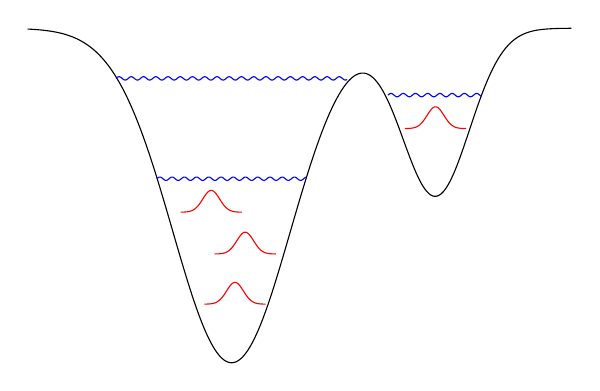
\begin{tikzpicture}
	\def\lims{xmin=-6,xmax=10,ymin=-2.1,ymax=0.01}
    \begin{axis}[\lims,hide x axis, hide y axis,width=0.7\textwidth,height=0.5\textwidth]
	    \addplot[mark=none,samples=1000,domain=-10:10,y domain=-2.1:0.01] {-2*exp(-x*x/6)-1*exp(-(x-6)*(x-6)/2)};
	    \addplot[red,mark=none,samples=1000,domain=-0.8:1.0] {-1.65+0.13*exp(-49*(x-0.1)*(x-0.1)/6)};
	    \addplot[red,mark=none,samples=1000,domain=-0.5:1.3] {-1.35+0.13*exp(-49*(x-0.4)*(x-0.4)/6)};
	    \addplot[red,mark=none,samples=1000,domain=-1.5:0.3] {-1.1+0.13*exp(-49*(x+0.6)*(x+0.6)/6)};
	    \addplot[blue,mark=none,samples=1000,domain=-2.2:2.2] {-0.9+0.01*sin(1000*(x+2.2))};
	    \addplot[blue,mark=none,samples=1000,domain=-3.4:3.4] {-0.3+0.01*sin(1000*(x+3.4))};
	    
	    \addplot[red,mark=none,samples=1000,domain=5.1:6.9] {-0.60+0.13*exp(-49*(x-6.0)*(x-6.0)/6)};
	    \addplot[blue,mark=none,samples=1000,domain=4.6:7.35] {-0.4+0.01*sin(1000*(x-4.6))};
	\end{axis}
	\end{tikzpicture}
	\caption{A schematic representation of metadynamics. The free energy well is gradually filled up with small Gaussians, and a transition is facilitated.}\label{Fig:ES:metadynamics}
\end{figure}

%\begin{figure}[htbp]
%	\centering
%	\includegraphics[width=0.8\textwidth]{figures/metadynamics.pdf}\\
%	\caption{A schematic representation of metadynamics. The free energy well is gradually filled up with small Gaussians, and a transition is facilitated.}\label{Fig:ES:metadynamics}
%\end{figure}

The above texts are merely an informal explanation of metadynamics. Formally, metadynamics belongs to a class of methods in which sampling is facilitated by introducing additional bias potential to pre-selected degrees of freedom, which are often referred as collective variables (CVs). In metadynamics, the bias potential added to the Hamiltonian of the system is history-dependent, and is often written as a sum of Gaussians deposited during the simulation as
\begin{equation}
   V_G(\mathbf{s},t) = \int\limits_0^t\diff t^\prime\, \omega\exp{\left(-\sum\limits_{i=1}^{d}\frac{\left[\mathbf{s}_i(R)-\mathbf{s}_i(R(t^\prime))\right]^2}{2\sigma_i^2}\right)}
\end{equation}
on a collective variable $\mathbf{s}$ in $d$-dimension. $\sigma$ and $\omega$ are two parameters tuning the shape of the Gaussians, which can be time-dependent. Asymptotically, 
\begin{equation}
   V_G(\mathbf{s},t\rightarrow \infty) = -F(\mathbf{s})+C.
\end{equation}

However, metadynamics suffers from several practical difficulties. First of all, it is often difficult to decide when to stop a metdynamics simulation. Practically, the free energy does not converge. Instead, it fluctuates around the correct values, leading to an average error proportional to the square root of the bias potential deposition rate. Furthermore, the system may be pushed into regions of configurational space not physically relevant in a long run. Recent improvement over the ordinary metadynamics on convergence issue, which is termed well-tempered metadynamics (WTMetaD), can be found in Ref.~\cite{BarducciPRL2008} and is reviewed in Ref.~\cite{ValssonARPC2016}. The idea of WTMetaD is that instead of completely filling the free energy well, it aims at enhancing the fluctuation of the CVs in a controllable manner. For instance, we can broaden the ensemble distribution by letting the biased probability distribution
\begin{equation}
	P_V(\mathbf{s})=\frac{[P(\mathbf{s})]^{1/\gamma}}{\int \diff \mathbf{s}^\prime[P(\mathbf{s}^\prime)]^{1/\gamma}},
	\label{Eq:ES:metadynamics:PvP}
\end{equation}
with $\gamma >1$. Taking the definition of the unbiased probability distribution $P(\mathbf{s})=\frac{\exp{[-\beta F(\mathbf{s})]}}{\int \exp{[-\beta F(\mathbf{s}^\prime)]} \diff\mathbf{s}^\prime}$ into the above equation, we find
\begin{align}
	P_V(\mathbf{s})=&\frac{\exp{[-\beta \frac{1}{\gamma}F(\mathbf{s})]}}{\int\diff \mathbf{s}^\prime \exp{[-\beta \frac{1}{\gamma}F(\mathbf{s}^\prime)]}}\notag\\
	               =&\frac{\exp{\left\{-\beta \left[F(\mathbf{s})-\left(1-\frac{1}{\gamma}\right)F(\mathbf{s})\right]\right\}}}{\int\diff \mathbf{s}^\prime \exp{\left\{-\beta \left[F(\mathbf{s}^\prime)-\left(1-\frac{1}{\gamma}\right)F(\mathbf{s}^\prime)\right]\right\}}}
\end{align}
where
$-\left(1-\frac{1}{\gamma}\right)F(\mathbf{s})$ is the biasing potential $V(\mathbf{s})$. The limit $\gamma \to 1$ corresponds to the unbiased ensemble.

If $\gamma \to \infty$ limit, then
\begin{equation}
	V(\mathbf{s})=-F(\mathbf{s})
\end{equation}
and
\begin{equation}
	P_V(\mathbf{s})=\frac{1}{\int \diff \mathbf{s}^\prime}=const,
\end{equation}
leading to a uniform distribution and the complete disappearance of the free energy barriers in the CV space, and the plain version of metadynamics is recovered.

Toward this end (Eq.~\ref{Eq:ES:metadynamics:PvP}), a gradually tempered Gaussian hill
\begin{equation}
    V_n(\mathbf{s})=V_{n-1}(\mathbf{s})+G(\mathbf{s},\mathbf{s}_n)\exp{\left[-\frac{1}{\gamma-1}\beta V_{n-1}(\mathbf{s}_n)\right]}
\end{equation}
is accumulated, where $V_0(\mathbf{s})=0$ and
\begin{equation}
    G(\mathbf{s},\mathbf{s}^\prime)=W\exp{\left(-||\mathbf{s}-\mathbf{s}^\prime||^2\right)}
\end{equation}
with $||\mathbf{s}-\mathbf{s}^\prime||^2$ being a distance metric such as
\begin{equation}
    ||\mathbf{s}-\mathbf{s}^\prime||^2=\frac{1}{2}\sum_{i,j}{(\mathbf{s}_i-\mathbf{s}_i^\prime)\Sigma_{i,j}^{-1}(\mathbf{s}_j-\mathbf{s}_j^\prime)}.
\end{equation}
$\Sigma_{i,j}^{-1}$ is the inverse of the covariance matrix $\Sigma_{i,j}$, and the latter is normally diagonal $\Sigma_{i,j}=\delta_{i,j}\sigma_i^2$. $W$ is the height of the Gaussian. $G(\mathbf{s},\mathbf{s}_n)$ is the biasing kernel centered on the current CV value $\mathbf{s}_n$ and is scaled by $\exp{\left[-\frac{1}{\gamma-1}\beta V_{n-1}(\mathbf{s}_n)\right]}$ when being accumulated. The scaling factor itself decreases as $1/n$, therefore the change of the biasing potential becomes smaller as the metadynamics simulation progresses.\cite{BarducciPRL2008,DamaPRL2014}

Practically, the update of the biasing potential is performed every $N_G$ steps. Between any two adjacent updates, the system evolves under the action of the biasing potential $V_n(\mathbf{s}(\mathbf{R}))$. After the $n$th update, the biasing potential is
\begin{equation}
    V(\mathbf{s},t)=\sum_{k=1}^n W\exp{\left(-||\mathbf{s}-\mathbf{s}_k||^2\right)}\exp{\left[-\frac{1}{\gamma-1}\beta V_{k-1}(\mathbf{s}_k)\right]}.
\end{equation}
The factor $(\gamma-1)\beta^{-1}$ is sometimes referred to as $k_B\Delta T$, or $\gamma=\frac{\Delta T+T}{T}$.

The remarkable feature of this stochastic update of the biasing potential is that the evolution of the bias can be described asymptotically by an ordinary differential equation (ODE)\cite{DamaPRL2014,TiwaryJCP2015}
\begin{equation}
    \frac{\diff V(\mathbf{s},t)}{\diff t}=\int \diff \mathbf{s}^\prime\, G(\mathbf{s},\mathbf{s}^\prime)\exp{\left[-\frac{1}{\gamma-1}\beta V(\mathbf{s}^\prime,t)\right]}P_V(\mathbf{s}^\prime,t),
\end{equation}
where
\begin{equation}
    P_V(\mathbf{s},t)=\frac{e^{-\beta[F(\mathbf{s})+V(\mathbf{s},t)]}}{\displaystyle\int \diff \mathbf{s}^\prime\, e^{-\beta[F(\mathbf{s}^\prime)+V(\mathbf{s}^\prime,t)]}}.
\end{equation}
For any $G(\mathbf{s},\mathbf{s}^\prime)$, this ODE has the asymptotic solution
\begin{equation}
    V(\mathbf{s},t)=-\left(1-\frac{1}{\gamma}\right)F(\mathbf{s})+c(t),
\end{equation}
where
\begin{equation}
    c(t)=\frac{1}{\beta}\log{\frac{\displaystyle\int \diff \mathbf{s}\, e^{-\beta F(\mathbf{s})}}{\displaystyle\int \diff \mathbf{s}\, e^{-\beta \left[F(\mathbf{s})+V(\mathbf{s},t)\right]}}}
    \label{Eq:ES:metadynamics:c}
\end{equation}
is independent of $\mathbf{s}$. Metadynamics thus converges to the desired result. Two interesting consequences arise.

First, it can be shown that, by taking the assumption of quasi-equilibrium, a time-dependent estimator for $F(\mathbf{s})$ is given by\cite{TiwaryJPCB2015}
\begin{equation}
    F(\mathbf{s})=-\left(\frac{\gamma}{\gamma -1}\right)V(\mathbf{s},t)+\frac{1}{\beta}\log{\int \diff \mathbf{s}\, \exp{\left[\frac{\gamma}{\gamma-1}\beta V(\mathbf{s},t)\right]}}.
    \label{eq:ES:metadynamics:FsFromBiasedPotential}
\end{equation}
Taking this equation into Eq.~\ref{Eq:ES:metadynamics:c}, one obtains
\begin{equation}
    c(t)=\frac{1}{\beta}\log{\frac{\displaystyle\int \diff \mathbf{s}\,\exp{\left[\frac{\gamma}{\gamma-1}\beta V(\mathbf{s},t)\right]}}{\displaystyle\int \diff \mathbf{s}\,\exp{\left[\frac{1}{\gamma-1}\beta V(\mathbf{s},t)\right]}}}.
\end{equation}
For a brief discussion on the calculations of $c(t)$, please refer to Ref.~\cite{GibertiJCTC2020}.

Second, it offers a practical way of calculating the expectation value of any $\mathbf{R}$-dependent function $O(\mathbf{R})$ as the simulation proceeds. The idea is that at time $t$ the biased probability distribution for $\mathbf{R}$ is given by
\begin{align}
    P_V{(\mathbf{R},t)}=&\frac{e^{-\beta\left[U(\mathbf{R})+V(\mathbf{s}(\mathbf{R}),t)\right]}}{\int \diff \mathbf{R}^\prime\, e^{-\beta\left[U(\mathbf{R}^\prime)+V(\mathbf{s}(\mathbf{R}^\prime),t)\right]}}\notag\\
                       =&\frac{e^{-\beta U(\mathbf{R})}e^{-\beta V(\mathbf{s}(\mathbf{R}),t)}\int e^{-\beta U(\mathbf{R^\prime})}\diff \mathbf{R}^\prime}{\int e^{-\beta U(\mathbf{R^\prime})}\diff \mathbf{R}^\prime \int e^{-\beta \left[U(\mathbf{R}^\prime)+V(\mathbf{s}(\mathbf{R}),t)\right]}\diff \mathbf{R}^\prime}\notag\\
                       =&P(\mathbf{R})\frac{e^{-\beta V(\mathbf{s}(\mathbf{R}),t)}\iint e^{-\beta U(\mathbf{R^\prime})}\delta (\mathbf{s}(\mathbf{R})-s)\diff \mathbf{R}^\prime \diff \mathbf{s}}{\iint e^{-\beta \left[U(\mathbf{R}^\prime)+V(\mathbf{s}(\mathbf{R}),t)\right]}\delta (\mathbf{s}(\mathbf{R})-s)\diff \mathbf{R}^\prime \diff \mathbf{s}}\notag\\
                       =&P(\mathbf{R})\frac{e^{-\beta V(\mathbf{s}(\mathbf{R}),t)}\int e^{-\beta F(\mathbf{s})}\diff \mathbf{s}}{\int e^{-\beta F(\mathbf{s})}e^{-\beta V(\mathbf{s},t)}\diff \mathbf{s}}\notag\\
                       =&P{(\mathbf{R})}e^{-\beta\left[V(\mathbf{s}(\mathbf{R}),t)-c(t)\right]},
\end{align}
where $P{(\mathbf{R})}=\frac{e^{-\beta U(\mathbf{R})}}{\int e^{-\beta U(\mathbf{R}^\prime)}\diff \mathbf{R}^\prime}$ is the unbiased Boltzmann distribution, and $e^{\beta\left[V(\mathbf{s}(\mathbf{R}),t)-c(t)\right]}$ is the time-dependent unbiasing factor. Here, $e^{-\beta c(t)}$ serves as a normalizing factor. Straightforwardly, the average of $O(\mathbf{R})$ over the unbiased ensemble can be calculated from the metadynamics trajectory as
\begin{equation}
    \left<O(\mathbf{R})\right>=\left<O(\mathbf{R})e^{\beta\left[V(\mathbf{s}(\mathbf{R},t)-c(t))\right]}\right>_V.
    \label{eq:ES:metadynamics:reweighting}
\end{equation}
This reweighting can be used to obtain the FES for some set of CVs $\mathbf{s}^\prime$ either biased or unbiased by setting $O(\mathbf{R})=\delta[\mathbf{s}^\prime-\mathbf{s}^\prime(\mathbf{R})]$. It is also useful if one chooses $\mathbf{s}^\prime$ as the biased degree of freedom $\mathbf{s}$ and obtain the FES. Disagreement between the FESs obtained directly from the bias potential (Eq.~\ref{eq:ES:metadynamics:FsFromBiasedPotential}) and through reweighting (Eq.~\ref{eq:ES:metadynamics:reweighting}) is a clear sign that the metadynamics simulation has not converged.

Metadynamics has been implemented in PLUMED (\url{https://plumed.github.io/doc-v2.3/user-doc/html/_metadyn.html}), which can work with major molecular dynamics packages.
\clearpage 
% !TeX spellcheck = en_US
% !TeX encoding = UTF-8
\section{Variationally Enhanced Sampling Method\label{Sec:ES:VES}}
Variationally Enhanced Sampling (VES) method was developed by Valsson and Parrinello in 2014 an evolution of Metadynamic.\cite{ValssonPRL2014} It begins with the following functional of a bias potential $V(\mathbf{s})$
\begin{equation}
    \Omega[V]=\frac{1}{\beta} \ln \frac{\displaystyle\int \diff \mathbf{s}\, e^{-\beta[F(\mathbf{s})+V(\mathbf{s})]}}{\displaystyle\int \diff \mathbf{s}\, e^{-\beta F(\mathbf{s})}}+\int \diff \mathbf{s}\, p(\mathbf{s}) V(\mathbf{s}),
\end{equation}
where $p(\mathbf{s})$ is an arbitrary normalized probability distribution, and $F(\mathbf{s})$ is the unbiased free energy surface. This functional is convex and invariant under the addition of an arbitrary constant to $V(\mathbf{s})$, $\Omega[V+k]=\Omega[V]$. The potential that renders $\Omega[V]$ stationary is, with an constant,
\begin{equation}
    V(\mathbf{s})=-F(\mathbf{s})-(1/\beta)\ln{p(\mathbf{s})}
    \label{Eq:ES:VES:VFP}
\end{equation}
for $p(\mathbf{s})\neq 0$ and $V(\mathbf{s})=\infty$ otherwise. This stationary point is also the global minimum of $\Omega[V]$ since the functional is convex.

To make use of the variational property of $\Omega[V]$, the bias potential $V(\mathbf{s})$ is expanded as a function of a set of variational parameters $\boldsymbol{\alpha}=(\alpha_1,\alpha_2,\dots,\alpha_K)$, and then the function $\Omega(\boldsymbol{\alpha})=\Omega[V(\boldsymbol{\alpha})]$ is minimized with respect to $\boldsymbol{\alpha}$ until convergence is reached. With the converged potential $V(\mathbf{s};\boldsymbol{\alpha})$, the free energy surface $F(\mathbf{s})$ can be estimated from Eq.~\ref{Eq:ES:VES:VFP}.

The gradient $\Omega^\prime(\boldsymbol{\alpha})$
\begin{equation}
    \frac{\partial \Omega(\boldsymbol{\alpha})}{\partial \alpha_{i}}=-\left\langle\frac{\partial V(\mathbf{s} ; \boldsymbol{\alpha})}{\partial \alpha_{i}}\right\rangle_{V(\boldsymbol{\alpha})}+\left\langle\frac{\partial V(\mathbf{s} ; \boldsymbol{\alpha})}{\partial \alpha_{i}}\right\rangle_{p}
\end{equation}
and the Hessian $\Omega^{\prime\prime}(\boldsymbol{\alpha})$
\begin{align} 
    	\frac{\partial^{2} \Omega(\boldsymbol{\alpha})}{\partial \alpha_{j} \partial \alpha_{i}}=& \beta \operatorname{Cov}\left[\frac{\partial V(\mathbf{s} ; \boldsymbol{\alpha})}{\partial \alpha_{j}}, \frac{\partial V(\mathbf{s} ; \boldsymbol{\alpha})}{\partial \alpha_{i}}\right]_{V(\boldsymbol{\alpha})} \notag\\ &-\left\langle\frac{\partial^{2} V(\mathbf{s} ; \boldsymbol{\alpha})}{\partial \alpha_{j} \partial \alpha_{i}}\right\rangle_{V(\boldsymbol{\alpha})}+\left\langle\frac{\partial^{2} V(\mathbf{s} ; \boldsymbol{\alpha})}{\partial \alpha_{j} \partial \alpha_{i}}\right\rangle_{p} 
\end{align}
where $\left<\cdots\right>_{V(\boldsymbol{\alpha})}$ and $\operatorname{Cov}[\cdots]_{V(\boldsymbol{\alpha})}$ are the expectation value and the covariance, respectively, obtained in a biased simulation employing the potential $V(\boldsymbol{\mathbf{s};\alpha})$, and $\left<\cdots\right>_p$ is an expectation value in the distribution $p(\mathbf{s})$. A natural approach is to expand $V(\boldsymbol{\mathbf{s};\alpha})$ in a linear basis set and use the coefficient of this expansion as variational parameters,
\begin{equation}
     V(\boldsymbol{\mathbf{s};\alpha})=\sum_k\alpha_kG_k(\mathbf{s}).
\end{equation}
In this case the gradient and the Hessian simplify,
\begin{align}
    \frac{\partial \Omega(\boldsymbol{\alpha})}{\partial \alpha_{\mathrm{i}}}=&-\left\langle G_i(\mathbf{s})\right\rangle_{V(\boldsymbol{\alpha})}+\left\langle G_i(\mathbf{s})\right\rangle_{p},\\
    \frac{\partial^{2} \Omega(\boldsymbol{\alpha})}{\partial \alpha_j \partial \alpha_i}=&\beta \operatorname{Cov}\left[G_j(\mathbf{s}), G_i(\mathbf{s})\right]_{V(\boldsymbol{\alpha})}.
\end{align}
\clearpage 
\input {chapters/OSRW.tex}
\clearpage
% !TeX spellcheck = en_US
% !TeX encoding = UTF-8
\section{Enveloping Distribution Sampling\label{Sec:ES:EDS}}
Enveloping distribution sampling method was first proposed by Christ and van Gunsteren in 2007.\cite{ChristJCP2007}
When calculating the free energy difference between states $A$ and $B$,
\begin{equation}
	\Delta G_{BA}=G_B-G_A=-\beta^{-1}\ln{\frac{Q_B}{Q_A}},
\end{equation}
we may encounter convergence difficulty if the important spaces of these two states are well separated, shown as black lines in Fig.~\ref{Fig:ES:triple_gaussian}.
Simulation under the Hamiltonian of state $A$ can hardly cover the important region of Hamiltonian $B$, and then the free energy of state $B$ will be significantly overestimated.
\begin{figure}[htbp]
	\centering
	%	\resizebox{2cm}{!}{
	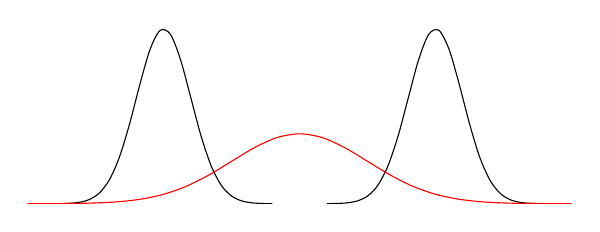
\begin{tikzpicture}
	\def\lims{xmin=-10,xmax=10,ymin=0.0001,ymax=0.6}
	\begin{axis}[\lims,hide x axis, hide y axis,width=0.7\textwidth,height=0.35\textwidth]
	    \addplot[mark=none,smooth,domain=-10:-1,y domain=0.0001:1] {0.5*exp(-(x+5)*(x+5)/2)};
		\addplot[mark=none,smooth,domain=1:10,y domain=0.0001:1] {0.5*exp(-(x-5)*(x-5)/2)};
		\addplot[color=red,mark=none,smooth,domain=-10:10,y domain=0.0001:1] {0.2*exp(-x*x/12.5)};
	\end{axis}
	\end{tikzpicture}
	%	}
	\caption{The configuration distributions under two Hamiltonians have no visible overlap as shown by solid black curves. A reference state (shown as the red curve) that has remarkable overlap with both states can be introduced to accelerate the convergence of the free energy calculations using, for instance, TP.}\label{Fig:ES:triple_gaussian}
\end{figure}

%\begin{figure}[htbp]
%	\centering
%	\includegraphics[width=0.6\textwidth]{figures/triple_gaussian.pdf}\\
%	\caption{The configuration distributions under two Hamiltonians have no visible overlap as shown by solid black curves. A reference state (shown as the red curve) that has remarkable overlap with both states can be introduced to accelerate the convergence of the free energy calculations using, for instance, TP.}\label{Fig:ES:triple_gaussian}
%\end{figure}
A simple solution to this difficulty is ``overlap sampling'', in which a reference state that can cover the important regions of both Hamiltonians $A$ and $B$ is introduced.
We then carry out a simulation for the reference state and the free energy difference between state $A$ and $B$ can be calculated as
\begin{equation}
	\Delta G_{BA}=\Delta G_{BR}-\Delta G_{AR}=-\beta^{-1}\ln{\dfrac{\langle e^{-\beta\left(H_B-H_R\right)}\rangle_R}{\langle e^{-\beta\left(H_A-H_R\right)}\rangle_R}},
\end{equation} 
which is a combination of two thermodynamic perturbation calculations from the reference state to the target states.

However, building the Hamiltonian of the reference state is not trivial. Without knowledge of the Hamiltonians for state $A$ and state $B$, we cannot generate an effective Hamiltonian,
especially in a high dimensional space. Enveloping distribution sampling method provides a natural way to generate the reference state, of which the configurational integral is the sum of the configurational integral of state A and B
\begin{align}
	Z_R=&Z_A+Z_B\notag\\
	   =&\int \left(e^{-\beta H_A(\mathbf{r})}+e^{-\beta H_B(\mathbf{r})}\right) \diff \mathbf{r}.
\end{align}
Correspondingly, the Hamiltonian is
\begin{equation}
	H_R(\mathbf{r})=-\beta^{-1}\ln{\left(e^{-\beta H_A(\mathbf{r})}+e^{-\beta H_B(\mathbf{r})}\right)}.
\end{equation}
A more general form can be written as
\begin{equation}
	H_R(\mathbf{r})=-\left(s\beta\right)^{-1}\ln{\left(e^{-s\beta H_A(\mathbf{r})}+e^{-s\beta H_B(\mathbf{r})}\right)},
	\label{Eq:ES:EDS:H_R}
\end{equation}
where $s$ is a scale factor that modulates the mixing\cite{ChristJCTC2009} as shown in Fig.~\ref{Fig:ES:EDS}. Increasing $s$ lowers the barrier height separating the two minima in the mixed potential, thereby enhances the transition. Straightforwardly, you may come to the idea that running Hamiltonian-REMD with different $s$ can remarkably increase the efficiency.
If you take a close look at Eq.~\ref{Eq:ES:EDS:H_R}, you will find that $s$ appears always with $\beta$. In other words, changing $s$ is equivalent to changing the temperature for the simulation. This is one interesting case where H-REMD and T-REMD are coincident with each other. 
\begin{figure}[htbp]
	\centering
	%	\resizebox{2cm}{!}{
	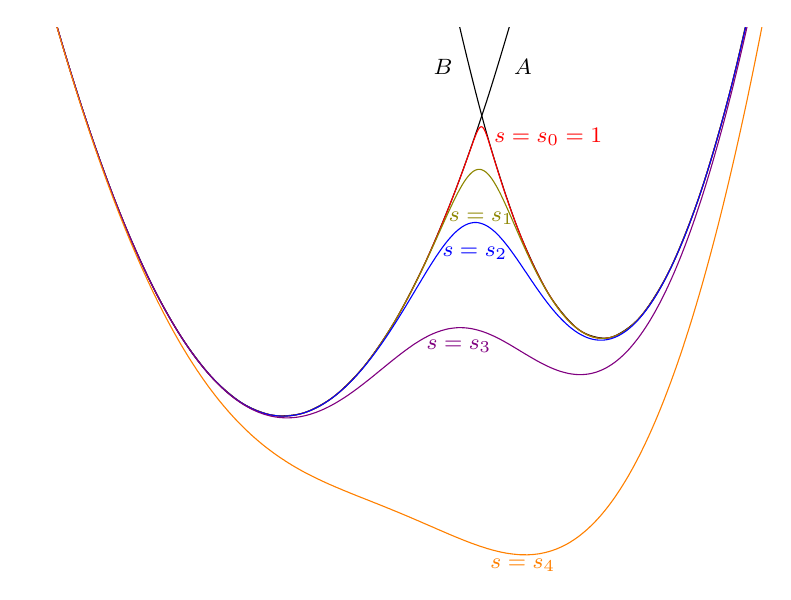
\begin{tikzpicture}[
	declare function={ f0(\x)=pow((\x+5),2);
		               f1(\x)=10+2*pow((\x-5),2);
 		               fR(\x,\s)=-1.0/(0.5*\s)*ln(exp(-0.5*\s*f0(\x))+exp(-0.5*\s*f1(\x)));
	},
	]
	\def\lims{xmin=-13,xmax=10,ymin=-20,ymax=50}
	\begin{axis}[\lims,hide x axis, hide y axis,width=0.9\textwidth,height=0.7\textwidth]
	\addplot[mark=none,smooth,domain=-13:10] {f0(x)};
	\addplot[mark=none,smooth,domain=-13:10] {f1(x)};
	\addplot[color=red,mark=none,samples=500,domain=-13:10] {fR(x,1.0)};
	\addplot[color=olive,mark=none,samples=500,domain=-13:10] {fR(x,0.2)};
	\addplot[color=blue,mark=none,samples=500,domain=-13:10] {fR(x,0.1)};
	\addplot[color=violet,mark=none,samples=500,domain=-13:10] {fR(x,0.05)};
	\addplot[color=orange,mark=none,samples=500,domain=-13:10] {fR(x,0.025)};
    \node[] at (axis cs: 2.5,45) {\footnotesize$A$};
    \node[] at (axis cs: 0.0,45) {\footnotesize$B$};
    \node[color=red] at (axis cs: 3.3,36) {\footnotesize$s=s_0=1$};
    \node[color=olive] at (axis cs: 1.2,25.5) {\footnotesize$s=s_1$};
    \node[color=blue] at (axis cs: 1.0,21) {\footnotesize$s=s_2$};
    \node[color=violet] at (axis cs: 0.5,9) {\footnotesize$s=s_3$};
    \node[color=orange] at (axis cs: 2.5,-19.2) {\footnotesize$s=s_4$};
	\end{axis}
	\end{tikzpicture}
	%	}
	\caption{State A and state B have only negligible overlap at high energy regions. The reference state generated by the mixing of state A and state B is tuned by $s$. Increasing $s$ may lower the barrier between the dominant wells. $s_0, s_1, s_2, s_3, s_4 = 1.0, 0.2, 0.1, 0.05, 0.025$.}\label{Fig:ES:EDS}
\end{figure}

%\begin{figure}[htbp]
%	\centering
%	\includegraphics[width=0.8\textwidth]{figures/EDS.pdf}\\
%	\caption{State A and state B have only negligible overlap at high energy regions. The reference state generated by the mixing of state A and state B is characterized by $s$. Increasing $s$ may lower the barrier between the dominant wells.}\label{Fig:ES:EDS}
%\end{figure}

The force is also a mixing quantity from two Hamiltonians as
\begin{align}
	\mathbf{F}_R^i=-\frac{\partial H_R}{\partial \mathbf{r}^i}=&\frac{e^{-s\beta H_A(\mathbf{r})}}{e^{-s\beta H_A(\mathbf{r})}+e^{-s\beta H_B(\mathbf{r})}}\left(-\frac{\partial H_A(\mathbf{r})}{\partial \mathbf{r}^i}\right)\notag\\
	&+\frac{e^{-s\beta H_B(\mathbf{r})}}{e^{-s\beta H_A(\mathbf{r})}+e^{-s\beta H_B(\mathbf{r})}}\left(-\frac{\partial H_B(\mathbf{r})}{\partial \mathbf{r}^i}\right).
\end{align}

A slight extension of the original EDS implementation reads
\begin{equation}
	H_R(\mathbf{r})=-\left(s\beta\right)^{-1}\ln{\left(e^{-s\beta (H_A(\mathbf{r})-F_A)}+e^{-s\beta (H_B(\mathbf{r})-F_B)}\right)},
	\label{Eq:ES:EDS:H_Rext}
\end{equation}
where $F_A$ and $F_B$ are the (free) energy offsets. With this new functional form, the mixed state looks like
\begin{figure}[htbp]
	\centering
	%	\resizebox{2cm}{!}{
	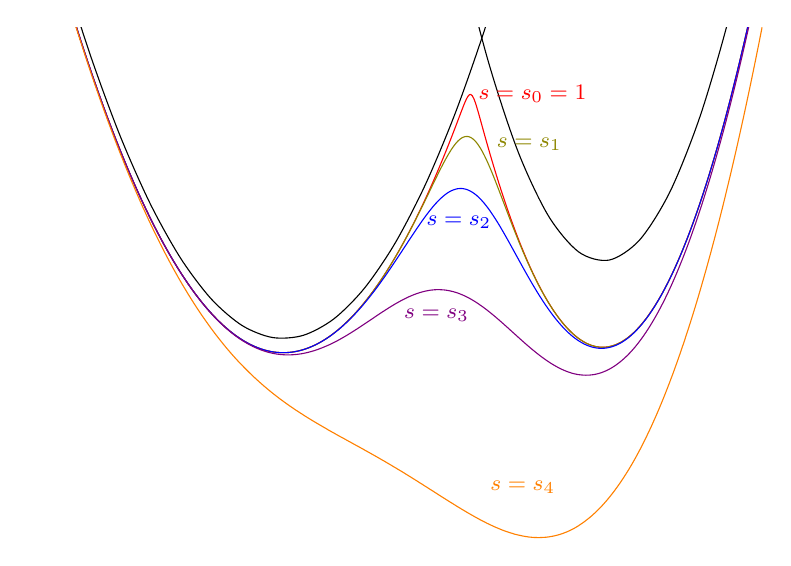
\begin{tikzpicture}[
	declare function={ f0(\x)=(\x+5)*(\x+5);
		f1(\x)=10+2*(\x-5)*(\x-5);
		fR(\x,\s)=-1.0/(0.5*\s)*ln(exp(-0.5*\s*(f0(\x)-1.84))+exp(-0.5*\s*(f1(\x)-10-1.14)));
	},
	]
	\def\lims{xmin=-13,xmax=10,ymin=-30,ymax=40}
	\begin{axis}[\lims,hide x axis, hide y axis,width=0.9\textwidth,height=0.7\textwidth]
	\addplot[mark=none,smooth,domain=-13:10] {f0(x)};
	\addplot[mark=none,smooth,domain=-13:10] {f1(x)};
	\addplot[color=red,mark=none,samples=500,domain=-13:10] {fR(x,1.0)};
	\addplot[color=olive,mark=none,samples=500,domain=-13:10] {fR(x,0.2)};
	\addplot[color=blue,mark=none,samples=500,domain=-13:10] {fR(x,0.1)};
	\addplot[color=violet,mark=none,samples=500,domain=-13:10] {fR(x,0.05)};
	\addplot[color=orange,mark=none,samples=500,domain=-13:10] {fR(x,0.025)};
	\node[] at (axis cs: 2.5,45) {\footnotesize$A$};
	\node[] at (axis cs: 0.0,45) {\footnotesize$B$};
	\node[color=red] at (axis cs: 2.8,31.5) {\footnotesize$s=s_0=1$};
	\node[color=olive] at (axis cs: 2.7,25.0) {\footnotesize$s=s_1$};
	\node[color=blue] at (axis cs: 0.5,15) {\footnotesize$s=s_2$};
	\node[color=violet] at (axis cs: -0.2,3) {\footnotesize$s=s_3$};
	\node[color=orange] at (axis cs: 2.5,-19.2) {\footnotesize$s=s_4$};
	\end{axis}
	\end{tikzpicture}
	%	}
	\caption{The reference state generated by the mixing of state A and state B tuned by $s$, $F_A$ and $F_B$. $s_0, s_1, s_2, s_3, s_4 = 1.0, 0.2, 0.1, 0.05, 0.025$.}\label{Fig:ES:EDS_ext}
\end{figure}

Interestingly, the idea of EDS can be dated back to the early work by Han\cite{HanPRA1992}, of which the best estimate of $s$ is 2. For a more rigorous deviation, please refer to Christ.\cite{ChristJCP2008}

Recently, K\"onig et al proposed $\lambda$-EDS method\cite{KonigJCIM2020}, in which the reference (intermediate) Hamiltonian reads
\begin{align}
	H_{\lambda-EDS}=-[\beta s(\lambda)]^{-1}\ln\left\{(1-\lambda)e^{-\beta s(\lambda)H_A}+\lambda e^{-\beta s(\lambda)[H_B-E(\lambda)]}\right\}.
\end{align}
In this definition, the parameter $s$ is also a function of $\lambda$. It returns to EDS with $\lambda=0.5$, and returns to the minimum variance pathway (MVP) method\cite{BlondelJCC2004} with $s=0.5$ and $E=\Delta G_{A\rightarrow B}$. With this definition of intermediate states, it can replace soft-core potentials\cite{ZachariasJCP1994} used in alchemical transformations.
%\clearpage
%\input chapters/NEB.tex
\clearpage
\input {chapters/string.tex}
\clearpage
\input {chapters/OAMS.tex}
